\documentclass{letnab}

\newtheorem*{determenition}{Определение}
\newcommand{\p}{\partial}

\rhead{Гармонический анализ МФТИ}
\lhead{Экзамен}
\renewcommand{\headrulewidth}{2pt}


\usepackage{xcolor,colortbl}

\newcommand{\mc}[2]{\multicolumn{#1}{c}{#2}}
\newcommand{\und}{\;\&\;}
\definecolor{Gray}{gray}{0.85}
\definecolor{LightCyan}{rgb}{0.88,1,1}

\newcolumntype{g}{>{\columncolor{Gray}}X[c]}

\usepackage{tabularx,environ}

\definecolor{urlcolor}{HTML}{0000FF} % цвет гиперссылок

\hypersetup{pdfstartview=FitH, urlcolor=urlcolor, colorlinks=true}

\NewEnviron{greySmth}[1]
{\begin{table}[H]
		\begin{tabularx}{\textwidth}{>{\columncolor{Gray}}p{6.4em}  >{\columncolor{Gray}}X}
			#1 & 
		\BODY
		\end{tabularx}
	\end{table}
}

\NewEnviron{greyDefinition}
{\begin{table}[H]
		\begin{tabularx}{\textwidth}{>{\columncolor{Gray}}p{06.4em}  >{\columncolor{Gray}}X}
			\begin{definition}
			\end{definition} & 
			\BODY
		\end{tabularx}
	\end{table}
}

\NewEnviron{greyTheorem}
{\begin{table}[H]
		\begin{tabularx}{\textwidth}{>{\columncolor{Gray}}p{6.4em}  >{\columncolor{Gray}}X}
			\begin{theorem}
			\end{theorem} & 
			\BODY
		\end{tabularx}
	\end{table}
}


\NewEnviron{greyProof}
{\begin{table}[H]
		\begin{tabularx}{\textwidth}{>{\columncolor{Gray}}p{0.5em} X}
			$ \! $ & \textbf{Доказательство.} \newline
		\BODY
		\end{tabularx}
	\end{table}
}

\NewEnviron{greyEmpty}
{\begin{table}[H]
		\begin{tabularx}{\textwidth}{>{\columncolor{Gray}}p{0.5em} X}
			$ \! $ & 	
			\BODY
		\end{tabularx}
	\end{table}
}

\begin{document}
	\begin{titlepage}
\center % Center everything on the page
 
%----------------------------------------------------------------------------------------
%	HEADING SECTIONS
%----------------------------------------------------------------------------------------

\textsc{\LARGE Московский Физико-Технический Институт}\vspace{-15pt}\\[1cm] % Name of your university/college
\textsc{\Large Кафедра высшей математики}\\[0.5cm] % Major heading such as course name


%----------------------------------------------------------------------------------------
%	TITLE SECTION
%----------------------------------------------------------------------------------------

\HRule
\\[0.4cm]
{ \huge \bfseries Гармонический анализ}
\\[0.2cm] % Title of your document
\HRule
\\[1.5cm]


 
%----------------------------------------------------------------------------------------
%	AUTHOR SECTION
%----------------------------------------------------------------------------------------
\textsc{\Large  Экзамен}\\[2cm]


\includegraphics[width = 65 mm]{BOTAY.png}\\

Автор: \href{https://vk.com/domrachev_alexey}{\textsc{Домрачев Алексей}}\\














\begin{bottompar}
\begin{flushright} \large
		
\textit{при поддержке студсоветов ФРТК и ФУПМ}\\

\end{flushright}


\begin{center}	
	
\includegraphics[width = 80 mm]{logo.jpg}
	
\end{center}
\end{bottompar}
\end{titlepage}


	\tableofcontents
	\newpage
	\section{Теорема Римана. Стремление к нулю коэффициентов Фурье.} 
%\subsection{Пространства интегрируемых функций.}
$ X = \{a,b\}: [a,b],(a,b),[a,b), (a,b] $, может быть $ a = - \infty,\; b = +\infty $, $ X $ --- промежуток.
\begin{greyDefinition}Функция $ y = f(x) $ называется абсолютно интегрируемой на промежутке $ X $, если $ \int_X \abs{f}dx $ сходится.
\end{greyDefinition}

\begin{greySmth}{Обозначения.} Совокупность абсолютно интегрируемых функций обозначается $ L^1_R(X) $
\end{greySmth}
\paragraph{Замечание} Если $ f $ интегрируема на $ [a,b] $, то $ \abs{f} $ --- интегрируема на $ [a,b] $. В обратную сторону утверждение неверно, пример функция Дирихле не интегрируема в общем случае, но интегрируема по модулю.
$$ {\widetilde{\mathcal{D}}(x)} = \begin{cases}
1&, x \in \mathbb{Q}\\ -1&, x \in \mathbb{J}
\end{cases} $$ 
\paragraph{Замечание.} На $ L^1_R(X) $ можно определить операции сложения функций и умножения функции на действительное число. Тем самым $ L_R^1(X) $ превращается в линейное пространство.
\begin{greyDefinition} Функция $ f \in L^1_R(X) $ называется абсолютно интегрируемой с квадратом, если $ \int_X \abs{f}^2dx $ сходится. Множество таких функций обозначают $ L^2_R(X) $ $$ \abs{f}^2 \in L^1_R(X) \Rightarrow f \in L^2_R(X)$$ 
* -- $ f: X\rightarrow \mathbb{R} \Rightarrow \abs{f}^2 = f^2 $\newline
НО $ f: X \rightarrow \mathbb{C} \Rightarrow \abs{f}^2 \neq f^2 $ 
\end{greyDefinition}

\paragraph{Пример.} $ f(x) = \frac{1}{\sqrt{x}}, \; X = (0,1],\; f \in L^1_R(X),\; f^2 \notin L^1_R(X) $
\paragraph{Предложение.} $ L^2_R(X) $ --- линейное пространство.

\paragraph{Определение.} Линейное пространство $ L $ называется нормированным пространством, если на $ L $ введена функция $ ||\cdot|| $ называемая нормой, обладающая следующими свойствами $ (\forall x,y \in L\; \& \forall \alpha \in \mathbb{R}) $
\begin{enumerate}
	\item $ ||x+y|| \leqslant ||x|| + ||y|| $
	\item $ ||\alpha x|| = |\alpha| ||x|| $
	\item $ ||x|| \geqslant0,\; ||x|| =0 \Leftrightarrow x = 0 $
\end{enumerate}

\begin{greyTheorem}
	\textbf{Теорема Римана об осцилляции}. Если $ f(x) $ абсолютно интегрируемая на конечном или бесконечном интервале $ (a,b) $: $ f \in L_R^1(X),\; X =\{ a,b \} $, то справедливо следующее равенство\[
	\lim\limits_{t\rightarrow\infty} \int_{a}^b f(x)\sin t xdx = 0;
	\]
	\[
	\lim\limits_{t\rightarrow\infty} \int_{a}^b f(x)\cos txdx = 0
	\]
\end{greyTheorem}
\begin{greyProof}
	\textit{Первый случай.} $ f $ --- интегрируемая на $ [a,b] $ функция. Критерий интегрируемости:
	\[
	\forall \varepsilon>0\, \exists T=\{ a = x_0<x_1<\ldots < x_k=b \}: \overline{S}_T-\underline{S}_T < \varepsilon/2
	\]
	Возьмем $ m_i=\inf_{[x_{i-1},x_i]} f,\; M_i=\sup_{[x_{i-1},x_i]} f,\; M=\sup_{[a,b]} |f| $.
	\begin{multline*}
	\left|\int_{a}^b f(x)\sin t xdx \right|= \left|\sum_{i=1}^{k} \int_{x_{i-1}}^{x_i}(f(x)-m_i)\sin t x dx + \sum_{i=1}^{k} m_i \int_{x_{i-1}}^{x_i} \sin t x dx\right|\leqslant\\\leqslant \sum_{i=1}^k (M_i-m_i)\Delta x_i + \sum_{i=1}^k \dfrac{m_i}{|t|}|\cos tx_{i-1} -\cos t x_i| \leqslant \\ \leqslant \sum_{i=1}^k (M_i - m_i) \Delta x_i + 2k\dfrac{M}{|t|} <  \varepsilon/2 + 2k\dfrac{M}{|t|}
	\end{multline*}
	Так как числа $ M \text{ и } k $ фиксированы, то
	\[
	\forall \varepsilon>0\,	 \exists t_0 > 0 : \forall t: |t|>t_0 \mapsto 2kM/|t|<\varepsilon/2 \mapsto \left|\int_{a}^b f(x)\sin t xdx \right| < \varepsilon,
	\]
	то есть $ \lim\limits_{t\rightarrow\infty} \int_a^b f(x)\sin tx dx = 0 $
	
	\textit{Второй случай.} $ X = [a,b),\,f  $ имеет особенность в точке $ b $.
	\[
	|f(x)\sin tx| \leqslant |f(x)| \Rightarrow f(x)\sin tx \in L_R^1(X) \Rightarrow\]
	Критерий Коши:
	\[	
	\forall \varepsilon>0 \exists \delta=\delta(\varepsilon) \in (0,b-a):\; \left|\int_{b-\delta}^{b} f(x)\sin t x dx \right| <\varepsilon/2
	\]
\end{greyProof}
\begin{greyEmpty}
	$ f $ интегрируема на $ [a,b-\delta] \Rightarrow$ из п. 1 $ \exists t_0>0: \forall t: |t| > t_0 \mapsto \left|\int_{a}^{b-\delta} f(x)\sin t x dx \right| <\varepsilon/2$
	 Поэтому при $ |t| > t_0 \mapsto  $
	\begin{multline*}
	\mapsto \abs{\int_{a}^{b} f(x) \sin tx dx } = \abs{\int_{a}^{b-\delta} f(x) \sin tx dx + \int_{b-\delta}^{b} f(x) \sin tx dx} \leqslant \abs{\int_{a}^{b-\delta} f(x) \sin tx dx} +\\+ \int_{b-\delta}^{b} |f(x)| \sin tx dx < \varepsilon/2 + \varepsilon/2 = \varepsilon
	\end{multline*}
	Итак, $ \lim\limits_{t \rightarrow \infty} \int_{a}^{b} f(x) \sin tx dx = 0$
\end{greyEmpty}
Косинус доказывается аналогично.
\begin{greyTheorem}
	Если $ f \in L_R^1(X),\; X =\{ -a,a \} $, четная на $ X $, то \[
	\int_{-a}^{a} f(x)dx = 2 \int_{0}^{a} f(x)dx
	\]
	Если $ f $ нечетная на $ X $, то \[
	\int_{-a}^a f(x)dx = 0
	\]
\end{greyTheorem}
%не доказано
\begin{greyTheorem}
	Если $ f \in L_R^1(X), X = \{ 0,T \} $, и периодическая с периодом $ T $ продолжена на $ \mathbb{R} $, то $ f$ абсолютно интегрируема на любом отрезке конечной длины и $ \forall a \in \mathbb{R} $\[ \int_{a}^{a+T} f(x)dx = \int_{0}^T f(x)dx \]
\end{greyTheorem}
%не доказано

\textbf{Тригонометрические ряды Фурье.}

\begin{greySmth}{Замечание.}
	В теории тригонометрических рядов Фурье принята запись
	\[
	a_0 = \dfrac{1}{l} \int_{-l}^l f(x)dx,\; a_k =\dfrac{1}{l} \int_{-l}^lf(x) \cos\dfrac{k\pi x}{l},\; b_k=\dfrac{1}{l} \int_{-l}^l f(x) \sin \dfrac{k \pi x}{l}
	\]
\[
\frac{a_0}{2} + \sum_{k=1}^\infty a_k\cos \dfrac{k\pi x}{l} + b_k \sin \dfrac{k\pi x}{l} \sim f(x) \text{ --- Ряд Фурье}
\]
\end{greySmth}

\begin{greySmth}{Замечание 1.}
	Так как 
	$
	\left|f(x) \cos \dfrac{k \pi x}{l} \right| \leqslant |f(x)| \& \left|f(x)\sin \dfrac{k\pi x}{l}\right| \leqslant |f(x)| \Rightarrow$  несобственные интегралы, задающие  $a_k$ \text{ и } $b_k$ \text{ сходятся}.
\end{greySmth}

\begin{greySmth}{Замечание 2.}
	Из т. Римана об осцилляции следует, что $ a_k \rightarrow 0,\; b_k \rightarrow 0,\text{ при } k \rightarrow \infty $
\end{greySmth}


\paragraph{Замечание 3.} Функцию $ f \in  \mathcal{L}_R^2[-l,l]$ периодически с периодом $ 2l $ продолжим на $ \mathbb{R} $. По теореме об интеграле периодической функции продолженная функция будет абсолютно интегрируема на любом конечном интервале. Если $ f $ непрерывна на $ [-l,l] $ и $ f(-l+0)=f(l-0) $, то продолженная функция будет непрерывна на всей числовой оси. Если эти пределы не совпадают, то в т. $ (2m+1)l,\; m\in \mathbb{Z} $ --- точка разрыва 1-го рода со скачком $ f(-l+0)-f(l-0) $
	\newpage
	\section{Представление частичной суммы ряда Фурье интегралом через ядро Дирихле. Принцип локализации.}
Будем рассматривать такие функции: $ f \in L_R^1[-l,l] $
\begin{greyDefinition}Функцию
	\[
	D_n(u) = \dfrac{1}{2} + \sum_{k=1}^n \cos ku
	\]
	называют ядром Дирихле
\end{greyDefinition}
Запишем частичную сумма ряда Фурье в подходящем виде:
\begin{multline*}
	S_n^f = \dfrac{a_0}{2} + \sum_{k=1}^n \left(a_k \cos \dfrac{k\pi x}{l} + b_k \sin \dfrac{k\pi x}{l}\right)= \\ = \dfrac{1}{2l} \int_{-l}^l f(t)dt +  \sum_{k=1}^n \Bigg( \left[ \dfrac{1}{l} \int_{-l}^l f(t)\cos \dfrac{k\pi t}{l} dt \right] \cos \dfrac{k\pi x}{l} + \left[ \dfrac{1}{l} \int_{-l}^l f(t) \sin \dfrac{k\pi t}{l}dt \right] \sin \dfrac{k\pi x}{l} \Bigg) =\\= \dfrac{1}{l} \int_{-l}^l f(t) \left[ \dfrac{1}{2} + \sum_{k=1}^n \left( \cos \dfrac{\pi k t}{l} \cos \dfrac{\pi k x}{l} + \sin \dfrac{\pi k t}{l} \sin \dfrac{\pi k x}{l} \right) \right]dt = \\ =\dfrac{1}{l} \int_{-l}^l f(t) \left[ \dfrac{1}{2} + \sum_{k=1}^n \cos \dfrac{k\pi (t-x)}{l} \right]dt = \dfrac{1}{l} \int_{-l}^{l} f(t) D_n dt
\end{multline*}
\begin{greySmth}{Свойства.}
\textbf{Свойства ядра Дирихле:}
\begin{enumerate}
	\item $ D_n (u) = D_n(-u) $ --- функция четная
	\item $ D_n(u+2\pi) = D_n(u) $ --- функция периодическая с периодом $ 2\pi $
	\item $ D_n(u)  $ --- непрерывная на $ \mathbb{R} $ функция
	\item $ D_n(u) = \dfrac{\sin (n+1/2)u}{2\sin u/2},\; u \neq 2\pi m\; \forall m \in \mathbb{Z} $, НО \[
	\lim\limits_{u \rightarrow 0} D_n(u) = (n+\frac{1}{2})
	\]
	\item $ \int_{-\pi}^{\pi} D_n(x)dx = \pi \overset{\text{Св. 1}}{\Longrightarrow} \int_{0}^{\pi} D_n(x) dx= \pi/2,\; \forall l \mapsto \int_{0}^{l} D_n\left(\dfrac{\pi}{l}y\right)dy = l/2 $
\end{enumerate}
\end{greySmth}
\begin{greyProof} Свойство 4.
	\begin{multline*}
		D_n(u) \sin \frac{u}{2} = 1/2 \sin \frac{u}{2} + \sum_{k=1}^n \cos ku \sin \frac{u}{2} = 1/2 \sin \frac{u}{2} + 1/2\sum_{k=1}^n \sin (k+1/2)u - \sin (k-1/2)u =\\= 1/2 \sin (n+1/2)u
	\end{multline*}%какая-то лажа
\end{greyProof}

Выведем Формулу Дирихле.
\begin{greyProof}
\text{Итак:}
\begin{multline*}
	S_n^f(x) = \frac{1}{l} \int_{-l}^l f(t) D_n\left(\frac{\pi}{l}(t-x)\right)dt = \frac{1}{l} \int_{x-l}^{x+l} f(t) D_n\left(\frac{\pi}{l}(t-x)\right)dt = \\
	\left|	\begin{array}{c} \rowcolor{red!20} t-x = z,\; dt=dz,\; t=x+l,\;z=l \\ \rowcolor{Gray} t=x+z;\; z= -l\end{array}\right| \\
	= \frac{1}{l} \int_{-l}^0 f(x+z)D_n\left(\frac{\pi}{l}z\right)dz + \frac{1}{l}\int_{0}^l f(x+z) D_n\left(\frac{\pi}{l}z\right)dz = \\ | z = -S | \\ = \frac{1}{l} \int_{0}^lf(x-S) D_n\left( - \frac{\pi}{l}S\right)dS + \frac{1}{l} \int_{0}^l f(x+z) D_n\left(\frac{\pi}{l}z\right)dz \Rightarrow
\end{multline*}
\[
	\Rightarrow	S_n^f(x) = \frac{1}{l} \int_{0}^l \left[ f(x+z) + f(x-z) \right] D_n\left(\frac{\pi}{l}z\right)dz
\]
\end{greyProof}
\textbf{ \large Принцип локализации.}
\begin{greyTheorem}
	Пусть функция $ f \in L_R^1[-l,l]$ продолжена с периодом $ 2l $ на $ \mathbb{R} $. Тогда сходимость тригонометрического ряда Фурье функции $ f $ в произвольной точке $ x_0 $ и сумма этого ряда в точке $ x_0 $ (если ряд сходится в т. $ x_0 $) зависят от поведения функции $ f $ в достаточно малой окрестности $ (x_0-\delta, x_0+\delta) $ т. $ x_0 $ при некотором $ \delta > 0 $.
\end{greyTheorem}
\begin{greyProof}
	При $ u \neq 2\pi k,\; k \in \mathbb{Z} $ справедливо тождество 
	\[
		D_n(u) = 1/2 + \cos u + \ldots + \cos nu = \dfrac{\sin (n+ 1/2)}{2 \sin u/2}
	\]
\end{greyProof}
\begin{greyEmpty}
	и формула Дирихле: $ S_n^f(x) = \frac{1}{l} \int_{0}^l \left[ f(x+u) + f(x-u) \right] D_n\left(\frac{\pi}{l}u\right)du $
	
	Запишем частичную сумму
 	\[
		S_n^f(x_0) = \frac{1}{l} \int_{0}^l \left[ \dfrac{ f(x_0+z) + f(x_0-z)}{2 \sin \dfrac{\pi}{2l}z} \right] \sin \left[ \frac{\pi}{l}(n+1/2)z \right]
	\]
	
	Так как $  f(x_0+z) + f(x_0-z) \in L_R^1 [-l,l] $ и 
	\[
		\forall z: \delta\in (0;z) \mapsto \dfrac{\abs{ f(x_0+z) + f(x_0-z)}}{2 \sin \dfrac{\pi}{2l}z} \leqslant \frac{\abs{ f(x_0+z) + f(x_0-z)}}{2\sin \dfrac{\pi\delta}{2l}} \Rightarrow 
	\]
	То по признаку сравнения функция $ F(z) = \dfrac{ f(x_0+z) + f(x_0-z)}{2\sin \dfrac{\pi}{2l}z} \in L_R^1[-l,l] $ абсолютно интегрируема на $ [ \delta, l] $. В силу теорему об осциляции:
	\[
		\Rightarrow \lim\limits_{n\rightarrow \infty} \frac{1}{l} \int_{\delta}^{l} F(z) \sin \left[ \dfrac{\pi}{l}(n+1/2)z \right]dz = 0 \Rightarrow 
	\]
	\[
		S_n^f(x_0) - \frac{1}{l} \int_{0}^\delta \dfrac{ f(x_0+z) + f(x_0-z)}{2\sin \dfrac{\pi z}{2l}} \sin \left[ \frac{\pi}{l}(n+1/2)z \right]dz \underset{n \rightarrow \infty}{\longrightarrow}0
	\]
	Это значит, что существование и величина предела $ \lim\limits_{n \rightarrow \infty} S_n^f(x_0)$ зависит только от существования и величины предела 
	\[
		\lim\limits_{n \rightarrow \infty} \dfrac{1}{l} \int_{0}^{\delta} \dfrac{f(x_0 + z) + f(x_0 - z) }{2 \sin \left[\dfrac{\pi z}{2l} \right]} \sin \left[\dfrac{\pi}{l}(n+1/2)z \right]dz
	\]
	То есть от значений функции $ f $ на интервале $ (x_0 - \delta, x_0 + \delta) $
\end{greyEmpty}

	\newpage
	\section{Достаточные условия сходимости ряда Фурье в \mbox{точке}.}
\begin{greyTheorem}
	\textbf{Признак Дини.} 	Пусть $ f \in L_R^1[-l,l] $ продолжена с периодом $ 2l $ на $ \mathbb{R} $, а $ S_0 $ --- такое число, что для некоторого $ \delta > 0,\; \delta \in (0,l)  $ сходится интеграл
	\[
		\int_0^\delta \dfrac{\abs{f(x_0+z) + f(x_0-z) -2S_0 }}{z} dz,
	\] 
	тогда ряд Фурье функции $ f $ сходится в точке $ x_0 $ к числу $ S_0 $: $$ S_n^f(x_0) \underset{n\rightarrow\infty}{\longrightarrow} S_0$$
\end{greyTheorem}
\begin{greyProof}
	$ \dfrac{f(x_0+z) + f(x_0-z) -2S_0}{z} \in L_R^1[0,l]$
	
	$$ \int_{-\pi}^{\pi} D_n(u)du = \int_{-\pi}^\pi \left( 1/2 + \cos u + \ldots + \cos nu \right) du =\pi,$$ в силу четности $$ \int_0^\pi D_n(u)du = \pi/2  \text{ и }  \int_{0}^{l} D_n \left(\dfrac{\pi z}{l} \right)dz = \dfrac{l}{2},$$ поэтому получим 
	$$
		S_0 = \dfrac{2}{l} \int_{0}^l S_0 D_n \left(\dfrac{\pi z}{l}\right)dz.
	$$
	В силу $$ S_n^f(x) = \dfrac{1}{l} \int_{0}^l \left(f(x+z) + f(x-z) \right) D_n\left(\frac{\pi}{l}z\right) dz $$
	\begin{multline*}
		S_n^f(x_0) -S_0 = \dfrac{1}{l} \int_{0}^l  \dfrac{f(x_0+z) + f(x_0-z)}{2\sin \frac{\pi}{2l}z} \sin \left[ \frac{\pi}{l}(n+1/2)z \right] dz - S_0 \frac{2}{l} \int_{0}^l D_n\left(\frac{\pi}{l}z\right)dz = \\ = \frac{1}{l} \int_{0}^l \dfrac{f(x_0+z) + f(x_0-z)-2S_0}{2\sin \frac{\pi}{2l}z} \sin \left[ \frac{\pi}{l}(n+1/2)z \right] dz 
	\end{multline*}
	$$ g(z) = \dfrac{f(x_0+z) + f(x_0-z) - 2S_0}{z} \frac{z}{2\sin \dfrac{\pi}{2l}z}  $$
	 На отрезке $ [0,l] $ знаменатель обращается в 0 при $ z = 0 $, а $ \lim_{z\rightarrow 0} \dfrac{z}{2 \sin \frac{\pi z}{2 l }} = \dfrac{l}{\pi} $, поэтому функция $ \dfrac{z}{2\sin \left(\frac{\pi z}{2l} \right)} $ ограничена.
\end{greyProof}
\begin{greyEmpty}	 
 Так как $ g(z) \in L_R^1 [0,l] $, то по теореме Римана интеграл в правой части разности $ S_n^f(x_0) - S_0 $ стремится к нулю при $ n \rightarrow \infty $, т.е. $ S_n^f(x_0) - S_0 \underset{n \rightarrow \infty}{\longrightarrow} 0$, поэтому $$ \lim\limits_{n \rightarrow \infty} S_n^f(x_0) = S_0 $$
\end{greyEmpty}
\textbf{Признак Гельдера.}
\begin{greyDefinition} Функция $ y = f(x) $  в т. $ x_0 $ удовлетворяет условию Гельдера, если
 \begin{enumerate}
	\item существуют конечные значения $ f(x_0+0),\; f(x_0-0) $
	\item $ \exists \alpha \in (0,1],\; \exists C>0,\; \exists \delta> 0: \forall z \in (0,\delta) $
	
	$| f(x_0-z) - f(x_0-0) | \leqslant  Cz^\alpha$
	
	$ |f(x_0+z) - f(x_0+0) | \leqslant Cz^\alpha$
	
	$ \alpha $ --- показатель Гельдера, при $ \alpha=1 $ условие выше --- условие Липшица.
\end{enumerate}
\end{greyDefinition}
\begin{greySmth}{Введем.}
	Обобщенную левую производную:
$$f_-'(x_0) = \lim\limits_{z \rightarrow -0}\dfrac{f(x_0-z) - f(x_0-0)}{-z} $$
Обобщенную правую производную:
$$f_+'(x_0) = \lim\limits_{z \rightarrow +0} \dfrac{f(x_0+z)-f(x_0+0)}{z} $$
\end{greySmth}
\begin{greySmth}{Предложение.}
	Если у функции $ y=f(x) $ в точке $ x_0 $ существуют конечные обобщенные производные $ f_\pm'(x_0) $, то функция $ f $ в точке $ x_0 $ удовлетворяет условиям Липшица.
\end{greySmth}
\begin{greyProof}
	$ \exists \alpha \in (0,1],\; \exists C_{1,2}>0,\; \exists \delta> 0: \forall z \in (0,\delta) \mapsto
	\begin{cases}
	  \left| \dfrac{f(x_0-z)-f(x_0-0)}{-z}  \right| \leqslant C_1\\[0.9em]
	
	 \left| \dfrac{f(x_0+z)-f(x_0+0)}{z}  \right| \leqslant C_2
	 \end{cases}$
	 
	Тогда выберем $C = \max\{C_1,C_2\} \rightarrow$ условие Гельдера при $ \alpha = 1 $, т.е. условие \mbox{Липшица}.
\end{greyProof}
\paragraph{Следствие.} Если функция $ y=f(x) $ в т. $ x_0 $ имеет производную, то она в этой точке удовлетворяет условию Липшица.
\paragraph{Замечание.} В обратную сторону утверждение следствия неверно. Пример: $ y = |x| $ --- в т. $ x_0=0 $ удовлетворяет Липшицу, но не является дифференцируемой в этой точке.
\begin{greyTheorem}
	Пусть функция $ f \in L_R^1[-l,l] $ продолжена с периодом $ 2l $ на $ \mathbb{R} $ и в точке $ x_0 $ удовлетворяет условию Гельдера, тогда тригонометрический ряд Фурье функции $ f $  в точке $ x_0 $ сходится к $$ \dfrac{f(x_0+0)+f(x_0-0)}{2}. $$ Если кроме того, $ f $ непрерывна в т. $ x_0 $, то тригонометрический ряд \mbox{Фурье} функции $ f $ в этой точке сходится к $ f(x_0) $
\end{greyTheorem}
\begin{greyProof}
	Обозначим $ S_0 = \dfrac{f(x_0+0) + f(x_0-0)}{2} $
	\begin{multline*}
		\forall z \in (0,\delta) \mapsto \dfrac{\left| f(x_0+z) + f(x_0-z)-2S_0 \right|}{z} \leqslant \\ \leqslant \dfrac{\left| f(x_0+z) - f(x_0+0) \right|}{z} + \dfrac{\left| f(x_0-z) - f(x_0 - 0)\right|}{z}\leqslant \\ \leqslant \dfrac{Cz^\alpha + Cz^\alpha}{z} = \dfrac{2C}{z^{1-\alpha}},
	\end{multline*}
	Но так как $\alpha \in (0,1],\text{то } 1-\alpha \in [0,1) \Rightarrow $
	
	$$  \int_{0}^\delta \dfrac{dz}{z^{1-\alpha}}<\infty \overset{\text{пр. сравнения}}{\Longrightarrow}\int_{0}^\delta \dfrac{|f(x_0+z) + f(x_0-z) - 2S_0}{z}\, dz < \infty \overset{\text{пр. Дини}}{\Longrightarrow}$$
	\[ \Rightarrow S_n^f(x_0) \underset{n\rightarrow \infty}{\longrightarrow} S_0 = \dfrac{f(x_0+0)+ f(x_0-0)}{2} \]
\end{greyProof}
\begin{greySmth}{Следствие.} Пусть функция $ f \in L_R^1[-l,l] $ продолжена с периодом $ 2l $ на $ \mathbb{R} $ и в точке $ x_0 $ у нее существуют конечные $ f_\pm'(x_0) $, тогда тригонометрический ряд Фурье функция $ f $ в т. $ x_0 $ сходится к $ \dfrac{f(x_0+0) + f(x_0-0)}{2} $. Если же $ f $ дифференцируем в т. $ x_0 $, то тригонометрический ряд Фурье в той т. сходится к $ f(x_0) $.
\end{greySmth}
	\newpage
	\section{Дифференцирование и интегрирования рядов Фурье. Порядок убывания коэффициентов Фурье.}
\begin{greyDefinition}Функция $ y = f(x) $ называется \textbf{кусочно непрерывной} на отрезке $ [a,b] $, если $ \exists T = \{ a =x_0<x_1<\ldots<x_n=b \} $, такое что $ f $ непрерывно на $ (x_{i-1},x_i),\;i =\overline{1,n} $ и существует конечное $ f(a+0),\; f(x_i \pm 0),\; i =\overline{1,n},\; f(b-0) $
\end{greyDefinition}

Пример $y =  \begin{cases}
\text{sign}x, &x \in (-1,1)\\
0, &x = \pm 1 
\end{cases} $, продолжим с периодом 2 на $ \mathbb{R} \Rightarrow \forall [a,b]  $ содержит точку $ x = n,\; n \in \mathbb{Z} $, следовательно $ y $ --- кусочно непрерывная.

\begin{greyDefinition} Функция  $ y=f(x) $ называется \textbf{кусочно непрерывно дифференцируемой} на $ [a,b] $, если $ \exists T=\{ a=x_0<x_1<\ldots<x_n=b \} $, такие, что на $ [x_{i-1},x_i],\;i=\overline{0,n} $, функция $ f $ обладает непрерывными производными $ f' $, может быть с изменением значения функции $ f $ в точке $ x_k,\;k=\overline{1,n} $
\end{greyDefinition}
\begin{greyDefinition} Функция $ f $ называется \textbf{кусочно гладкой} на отрезке $ [a,b] $, если она непрерывна на отрезке $ [a,b] $ и кусочно непрерывно дифференцируема на нем.
\end{greyDefinition}

\paragraph{Замечание 1.} $ y=f(x) $ периодическая с периодом $ 2l $ на $ \mathbb{R} $
\[
	f(x+2l)=f(x) \Rightarrow f(-l) = f(l)
\]
и $ f $ кусочно гладкая на $ [-l,l] $, то $ f $ кусочно гладкая на любом $ [a,b] \subset \mathbb{R} $
\paragraph{Замечание 2.} Производная $ f' $ кусочно непрерывной дифференцируемой на $ [a,b] $ функции $ y = f(x) $ будет кусочно непрерывной на $ [a,b] $ функцией.
\paragraph{Замечание 3.} Тригонометрический ряд Фурье кусочно непрерывной дифференцируемой на $ [a,b] $ функции $  y = f(x)  $ в каждой точке непрерывности функции $ f $ сходится к $ f(x) $, а в точке разрыва $ x $ сходится к $ 1/2 \left[ f(x-0) + f(x+0) \right] $

\textbf{\large О почленном дифференцировании рядов Фурье.}
\begin{greyTheorem}
	Пусть $ y=f(x),\; 2l $--периодична на $ \mathbb{R} $ и кусочно гладкая на $ [-l,l] $, тогда тригонометрический ряд Фурье функции $ y=f'(x) $ получается из тригонометрического ряда Фурье функции $ f $ путем его почленного дифференцирования. 
\end{greyTheorem}
\begin{greyProof}
	\[
		f(x) \sim \dfrac{a_0}{2} + \sum_{k=1}^\infty a_k\cos \dfrac{k\pi x}{l} + b_k \sin \dfrac{k\pi x}{l}
	\]
	\[
		f'(x) \sim \dfrac{\overline{a_0}}{2} + \sum_{k=1}^\infty \overline{a_k}\cos \dfrac{k\pi x}{l} + \overline{b_k} \sin \dfrac{k\pi x}{l}
	\]
	\[
		\overline{a_0} = \dfrac{1}{l}\int_{-l}^l f'(x)dx= \dfrac{1}{l} (f(l)-f(-l)) =0
	\]
	\[
		\overline{a_k} = \dfrac{1}{l} \int_{-l}^lf'(x) \cos \dfrac{k\pi x}{l} dx = \dfrac{1}{l}\left[ f(x)\cos \dfrac{k\pi x}{l}\right|_{-l}^l + \dfrac{k\pi}{l} \left. \int_{-l}^lf(x)\sin \dfrac{k\pi x}{l} dx \right] = \dfrac{k\pi }{l} b_k
	\]
	\[
		\overline{b_k} = \dfrac{1}{l} \int_{-l}^l f'(x) \sin \dfrac{k\pi x}{l} dx = \dfrac{1}{l} \left[ f(x)\sin \dfrac{k\pi x}{l} \right|_{-l}^l - \dfrac{k\pi}{l} \left. \int_{-l}^lf(x)\cos \dfrac{k\pi x}{l} dx \right] = -\dfrac{k\pi}{l} a_k
	\]
	\textbf{Формальное дифференцирование} тригонометрического ряда Фурье функции $ f $ дает:
	\[
		\sum_{k=1}^\infty \fbox{$ -\dfrac{k\pi}{l}a_k $} \sin \dfrac{k\pi x}{l} + \fbox{$\dfrac{k\pi}{l}b_k$}\cos \dfrac{k\pi x}{l}
	\]
\end{greyProof}
\begin{greySmth}{Следствие.} Пусть $ f $ $ 2l $--периодическая на $ \mathbb{R} $ функция, имеет непрерывную производную на $ [-l,l] $ до порядка $ (m-2) $ включительно и кусочно гладкую производную порядка $ (m-1) $ на $ [-l,l] $, тогда тригонометрический ряд Фурье функции $ f^{(m)} $ получается из тригонометрического ряда Фурье функции $ f $ путем формального $ m $--кратного дифференцирования.
\end{greySmth}
\textbf{\large Асимптотические оценки коэффициентов Фурье.} 
\begin{greySmth}{Предложение 1.} Пусть функция $ y=f(x),\;2l $--периодическая на $ \mathbb{R} $ и кусочно гладкая на $ [-l,l] $, тогда для ее коэффициентов Фурье справедливы следующие асимптотические оценки:
\[
	a_n = o\left( \dfrac{1}{n} \right),\; b_n = o\left( \dfrac{1}{n} \right) \text{ при } n \rightarrow \infty 
\]
\end{greySmth}
\begin{greyProof}
	Следует из того, что коэф. Фурье производной $ f' $ равны $ \overline{a_k}  = \dfrac{\pi k}{l} b_k,\; \overline{b_k} = \dfrac{\pi k}{l}a_k$. Так как $ f' $ кусочно-непрерывна на $ [-l,l] $, то $ f' \in L_R^1[-l,l]  \Rightarrow $ по теореме Римана об осциляции $ \overline{a_k},\; \overline{b_k} $ стремятся к 0 при $ k \rightarrow \infty $
\end{greyProof}
\textbf{Вывод из предложения:} 
\[
	\overline{a_k} = \dfrac{\pi}{l} \dfrac{b_k}{\frac{1}{k}} \underset{k\rightarrow \infty}{\longrightarrow} 0,\quad \overline{b_k} = -\dfrac{\pi}{l} \dfrac{a_k}{\frac{1}{k}} \underset{k\rightarrow \infty}{\longrightarrow} 0
\]
\begin{greySmth}{Предложение 2.} Пусть $ f $ кусочно непрерывна дифференцируема на $ [-l,l] $ и периодически с периодом $ 2l $ продолжена на $ \mathbb{R} $. Тогда для коэффициентов Фурье функции $ f $ справедливо:
\[
	\exists C<0: \forall k \in \mathbb{N} \mapsto |ka_k| \leqslant C \,\&\, |kb_k| \leqslant C
\]
\[
	a_k = O \left( \dfrac{1}{k} \right),\quad b_k = O\left( \dfrac{1}{k} \right),\; k\rightarrow \infty
\]
\end{greySmth}
\begin{greyProof}
	\[
	\exists T = \{ -l=x_0<x_1<\ldots<x_n=l \}
	\]
	$ f $ непрерывно дифференцируема на $ [x_{k-1}, x_k],\; k = \overline{1,n} $. Тогда
\begin{multline*}	
		|ka_k| = \left| \dfrac{k}{l} \int_{-l}^l f(x) \cos \dfrac{k\pi x}{l} \right| = \left| \begin{array}{c} \rowcolor{red!20} f(x) = u \\ \cos \dfrac{k \pi x}{l}dx = dv  \end{array} \right|=\\= \dfrac{k}{l}\left|  \dfrac{l}{k\pi}f(x) \sin \dfrac{k\pi x}{l} \Big|_{-l}^l - \dfrac{l}{k\pi}\int_{-l}^l f'(x) \sin \dfrac{k \pi x}{l}dx  \right| =\\ =\dfrac{k}{l} \left| \sum_{i=1}^n \int_{x_{i-1}}^{x_i} f(x)\cos \dfrac{k\pi x}{l} dx  \right| = \\ = \dfrac{k}{l} \left| \sum_{i=1}^n \left[ \dfrac{l}{k\pi} f(x) \sin \dfrac{k\pi x}{l}\Big|_{x_{i-1}}^{x_i} - \dfrac{l}{k\pi} \int_{x_{i-1}}^{x_i} f'(x)\sin \dfrac{k\pi x}{l} dx \right] \right| \leqslant \\ \leqslant \dfrac{2}{\pi} \sum_{i=0}^{n} \left| f(x_i) \right| + \dfrac{1}{\pi} \left| \int_{-l}^l f'(x) \sin \dfrac{k\pi x}{l} dx \right|
\end{multline*}
$ \dfrac{2}{\pi} \sum_{i=0}^n |f(x_i)| = B,\, \exists A_1>0 \& A_2>0: \begin{matrix}
	\left|  \dfrac{1}{\pi} \int_{-l}^l f'(x) \sin \dfrac{k\pi x}{l} dx \right| \leqslant A_1\\[1em]	\left|  \dfrac{1}{\pi} \int_{-l}^l f'(x) \cos \dfrac{k\pi x}{l} dx \right| \leqslant A_2
\end{matrix}$

Тогда пусть $ C = \max\{B+A_1, B+A_2\} $, тогда $ |ka_k|\leqslant C  $ и $ |kb_k| \leqslant C $
\end{greyProof}
\begin{greySmth}{Следствие.} Пусть $ y=f(x),\; 2l$--периодическая на $ \mathbb{R} $ и на $ [-l,l] $ обладает непрерывной производной до порядка $ (m-2)  $ включительно и кусочно гладкой производной порядка $ (m-1) $. Тогда для коэффициентов Фурье функции $ f $ справедлива оценка:
\[
	a_k = o\left(\dfrac{1}{k^m}\right),\; b_k = o\left( \dfrac{1}{k^m} \right),\; k \rightarrow \infty
\]
\end{greySmth}
\begin{greyProof}
	\[
		f(x) \sim \dfrac{a_0}{2} + \sum_{k=1}^\infty a_k \cos \dfrac{k\pi x}{l} + b_k \sin \dfrac{k\pi x}{l}
	\]
	\[
		f^{(m)}(x) \sim \sum_{k=1}^\infty C_m a_k k^m \cos \left( \dfrac{k\pi x}{l} + m \dfrac{\pi}{2}\right) +C_m b_k k^m \sin \left( \dfrac{k\pi x}{l} + m\dfrac{\pi}{2} \right)
	\]
	\[
		C_m = \left( \dfrac{\pi}{l} \right)^m \left.:\begin{aligned}
		|a_kk^m | \rightarrow 0\\
		|b_kk^m| \rightarrow 0
		\end{aligned} \right\} k \rightarrow \infty
	\]
\end{greyProof}

\textbf{\large Почленное интегрирование рядов Фурье.}
\begin{greyTheorem}
	Пусть функция $ y=f(x) $ кусочно непрерывная на $ [-l,l],\;2l $--периодическая продолжена на $ \mathbb{R},\; f(x) \sim \dfrac{a_0}{2} + \sum_{k=1}^\infty a_k \cos \dfrac{k\pi x}{l} + b_k \sin \dfrac{k\pi x}{l} $ тогда тригонометрический ряд Фурье функции $ \Phi(x) =  \int_{0}^{x} f(t)dt - \dfrac{a_0x}{2} $ может быть получена путем формального интегрирования ряда Фурье функции $ f $.
\end{greyTheorem}
\begin{greyProof}
	$ F(x) = \int_{0}^{x} f(t)dt  $ --- кусочно гладкая на $ [-l,l] \Rightarrow \Phi(x)$ --- кусочно гладкая на $ [-l,l] $, т.к. $ \Phi(x) = F(x) - a_0x/2 $ имеет кусочно--непрерывную производную $ f(x) - a_0/2 $, причем $ \forall x: $
	\[
		\Phi(x+2l) - \Phi(x) = \int_{x}^{x+2l} f(t)dt - a_0l = \int_{-l}^l f(t)dt - a_0l = 0 \Rightarrow
	\]
	$ \Rightarrow \Phi\; 2l$--периодическая на $ \mathbb{R} $. Тогда по первой теореме этого пункта
	\[
		\Phi(x) \sim \dfrac{A_0}{2} + \sum_{k=1}^\infty A_k \cos \dfrac{k\pi x}{l} + B_k \sin \dfrac{k\pi x}{l}
	\]
	$ a_k = \dfrac{k\pi}{l} B_k,\; b_k = - \dfrac{k\pi}{l}A_k,\;\text{причем } \Phi(0)=0 \rightarrow \dfrac{A_0}{2} + \sum_{k=1}^\infty A_k = 0 \rightarrow\dfrac{A_0}{2} = \dfrac{l}{\pi} \sum_{k=1}^\infty \dfrac{b_k}{k} $
q\end{greyProof}
\begin{greyEmpty}
	\[
		\dfrac{l}{\pi} \left[ \sum_{k=1}^{\infty} \dfrac{b_k}{k} + \sum_{k=1}^\infty -\dfrac{b_k}{k}\cos \dfrac{k\pi x}{l} + \dfrac{a_k}{k} \sin \dfrac{k\pi x}{l}  \right] = \sum_{k=1}^\infty \dfrac{l}{\pi} \dfrac{b_k}{k} \left( 1- \cos \dfrac{k\pi x}{l}  \right) + \dfrac{l}{\pi} \dfrac{a_k}{k} \sin \dfrac{k\pi x}{l} 
	\]
	К такому же результату мы придем формально проинтегрировав ряд.
\end{greyEmpty}
\paragraph{Замечание.} $ f $ кусочно непрерывная на $ [-l,l] $ и $ 2l $--периодическая и продолжена на $ \mathbb{R} $, то для ее коэффициентов Фурье справедливо:
\[
	\sum_{k=1}^\infty \dfrac{b_k}{k} < \infty
\]
То есть $ \sum_{k=2}^\infty \dfrac{\sin \frac{k \pi x}{l}}{k} $ не может быть рядом Фурье никакой функции, так как расходится по интегральному признаку.
	\newpage	
	\section{Теорема о равномерной сходимости ряда Фурье.}

\begin{greyTheorem}
	Тригонометрический ряд Фурье $ 2l $--периодич. на $ \mathbb{R} $ и кусочно гладкой на $ [-l,l] $ функции $ f(x) $ сходится равномерно на $ \mathbb{R} $ к $ f $
\end{greyTheorem}
\begin{greyProof}
	1. Так как наша функция кусочно-гладкая, значит у неё существуют конечные значения справа и слева для каждой точки непрерывности, а также в силу кусочно-непрерывной дифференцируемости конечные значения производной справа и слева от неё, значит выполнено условие Липшица, значит выполнен признак Гельдера поточечной сходимости функции непрерывной к своему значению $ \Rightarrow $ ряд Фурье сходится к $ f $. 
	
	2. Теперь докажем равномерность.
	Воспользуемся неравенство Коши--Буняковского:
	\[
		\sum_{k=1}^n |a_k| = \sum_{k=1}^n  \abs{\dfrac{l}{k\pi} \overline{b_k}} \leqslant \dfrac{l}{\pi} \sqrt{\sum_{k=1}^n \dfrac{1}{k^2}} \sqrt{\sum_{k=1}^n (\overline{b_k})^2}
	\]
	\[
		\sum_{k=1}^n|b_k| \leqslant \dfrac{1}{\pi}\sqrt{\sum_{k=1}^n \dfrac{1}{k^2}} \sqrt{\sum_{k=1}^n (\overline{a_k})^2}
	\]
	Также $ f' \in L_R^1[-l,l] \Rightarrow$ \{ Неравенство Бесселя \} $ \sum_{i=1}^\infty \overline{a_k}^2\text{ и }\sum_{k=1}^\infty \overline{b_k}^2$ сходятся как и ряд $ \sum_{k=1}^\infty \dfrac{1}{k^2} $, а частные суммы этих рядов ограничены и $ \sum_{k=1}^n |a_k| \leqslant C, n =1,2,\ldots \Rightarrow $ по признаку сходимости $ \sum_{k=1}^\infty |a_k| < \infty $ и $ \sum_{k=1}^\infty |b_k| < \infty $
	\[
		\abs{a_k \cos \dfrac{k \pi x}{l} + b_k \sin\dfrac{k \pi x}{l}} \leqslant |a_k| + |b_k| \Rightarrow
	\] 
	$ \Rightarrow $ по признаку Вейерштрасса ряд Фурье $ f $ сходится равномерно на $ \mathbb{R} \text{ к } f $
\end{greyProof}
	\newpage
	\section{Равномерная сходимость сумм Фейера для непрерывной функции.}
\textbf{\large Сумма и ядро Фейера.}
\begin{greyDefinition}
	$ f  $ --- $ 2l $--периодическая и непрерывная на всей $ \mathbb{R} $, тогда сумма 
	\[
		\sigma_n(x) = \dfrac{S_0^f(x) + S_1^f(x) + \ldots + S_n^f (x) }{n+1} 
	\]
	называется \textbf{суммой Фейера}
	\[
		S_n^f(x) = \dfrac{1}{l} \int_{-l}^{l} f(x+z)D_n(\dfrac{\pi}{l}z)dz;\; \sigma_n(x) = \dfrac{1}{l} \int_{-l}^{l} f(x+z)F_n(z)dz
	\]
	\[
		F_n(z) = \dfrac{D_0(\frac{\pi}{l}z) + D_z(\frac{\pi}{l}z) + \ldots + D_n(\frac{\pi}{l}z)}{n+1} \text{ --- ядро Фейера}
	\]
\end{greyDefinition}
\begin{greyDefinition}
	Свойства ядра Фейера:\begin{enumerate}
		\item $ F_n $ --- $ 2l $--периодическая, четная и непрерывная на $ \mathbb{R} $ функция.
		\item $ \dfrac{1}{l} \int_{-l}^{l} F_n(z)dz = 1 $, т.к. $ \int_{0}^{l} D(\dfrac{\pi}{l}y)dy = l/2 $
		\item $ F_n(z) \geqslant 0 \forall z \in \mathbb{R} \left\{ F_n(u) = \dfrac{1}{2(n+1)} \left( \dfrac{\sin (n+1)\frac{\pi}{2l}u}{\sin \frac{\pi}{2l}u} \right)^2 \right\}$
		\item $ \forall \delta \in (0,l) \rightarrow \lim\limits_{n \rightarrow \infty} \max_{[\delta,l]} F_n(z) = 0;\;$ 
		
		$ \max F_n(z) \leqslant \dfrac{1}{2(n+1)\sin\frac{\pi}{2l}\delta} \underset{n \rightarrow\infty}{\longrightarrow}0$
	\end{enumerate}
\end{greyDefinition}
\begin{greyTheorem}
	Последовательность $ \left\{ \sigma_n(x) \right\}_{n=0}^\infty $ сумм Фейера $ 2l $--периодической и непрерывной на $ \mathbb{R} $ функции $ f $ сходится равномерно на $ \mathbb{R} $ к функции $ f $
\end{greyTheorem}
\begin{greyProof}
	\begin{enumerate}
		\item Докажем что $ f $ --- равномерно непрерывна на $ \mathbb{R} ;$ на $ [-2l,2l] $ функция $ f $ равномерно непрерывная по т. Кантора, т.е.\[
			\forall \varepsilon>0 \exists \delta >0: \forall x', x'' \in [-2l,2l]: |x'-x''| < \delta \mapsto |f(x') - f(x'')| < \varepsilon
		\]
		Возьмем произвольные любые $ \xi, \eta: |\xi - \eta| < \delta < l,\; x' \in [-l,l] $, тогда 
		\begin{multline*}
			\exists k: \xi = x' + 2kl, \eta = x'' + 2kl \Rightarrow |\xi - \eta| = |x' - x''|  < \delta \Rightarrow \\ \Rightarrow |f(\xi) - f(\eta)| = |f(x') - f(x'')| < \varepsilon
		\end{multline*}
		Условие равномерной непрерывности: $$ \forall \varepsilon > 0 \exists \delta = \delta(\varepsilon): \forall x \in \mathbb{R} \,\&\, \forall z: |z|<\delta \mapsto |f(x+z) - f(x)| < \frac{\varepsilon}{2} \Rightarrow  $$ $ \Rightarrow f $ --- равномерно непрерывна на $ \mathbb{R} $
		\[
			|\sigma_n(x) - f(x)| = |\frac{1}{l} \int_{-l}^l (f(x+z) - f(x)) F_n(z)dz| \leqslant \frac{1}{l} \int_{-l}^{l} |f(x+z)-f(x)| F_n(z)dz
		\]
		\[
			\frac{1}{l}\int_{-\delta}^{\delta} |f(x+z)-f(x)|F_n(z)dz \leqslant \frac{\varepsilon}{2}\frac{1}{l} \int_{-\delta}^\delta F_n(z)dz 
		\]
		По свойству $ \dfrac{1}{l} \int_{-l}^l F_n(z) dz = 1 $ и $ F_n(z) >0 \; \forall z \in \mathbb{R} \Rightarrow  \dfrac{1}{l}\int_{-a}^a F_n(z)dz < 1 \;\forall a<l $
		\[
			\Rightarrow \frac{\varepsilon}{2}\frac{1}{l} \int_{-\delta}^\delta F_n(z)dz < \frac{\varepsilon}{2}
		\]
		Введем $ M = \max_{[-l,l]} |f(x)|;\; \forall \varepsilon>0 \exists N=N(\varepsilon): \forall n \geqslant N \mapsto \max_{[-\delta,l]} F_n(z) \leqslant \dfrac{\varepsilon}{8M} $
		\[
			\frac{1}{l}\int_{\delta}^l |f(x+z)-f(x)|F_n(z) dz \leqslant \frac{1}{l}2M\frac{\varepsilon}{8M} (l-\delta) < \frac{\varepsilon}{4}
		\]
		\item Аналогично, $ \frac{1}{l}\int_{-l}^{\delta} |f(x+z)-f(x)|F_n(z)dz < \frac{\varepsilon}{4}$

		\item Тогда $ \abs{\sigma_n(x)-f(x)} = \frac{1}{l}\abs{\int_{-\delta}^\delta + \int_{\delta}^l + \int_{-l}^{-\delta}} < \frac{\varepsilon}{2} + \frac{\varepsilon}{4} + \frac{\varepsilon}{4} = \varepsilon$, т.е. 
		\[
			\forall \varepsilon > 0 \exists N(\varepsilon): \forall n \geqslant N \,\&\, \forall x \in \mathbb{R} \rightarrow |\sigma_n(x) - f(x)| < \varepsilon \Leftrightarrow \sigma_n(x) \tmb{x\in\mathbb{R}}{\rightrightarrows}{n \rightarrow\infty}f(x)
		\]
	\end{enumerate}
\end{greyProof}
	\newpage
	\section{Теоремы Вейерштрасса о приближении непрерывных функций тригонометрическими и алгебраическими членами.}
\[
	T_m(x) = A_0 + \sum A_k \cos \dfrac{k\pi x}{l} + B_k \sin \dfrac{k \pi x}{l}\text{ --- тригоном. многочлен}
\]
\begin{greyTheorem}
	\textbf{Теорема Вейерштрасса.} Любую $ 2l $--периодическую непрерывную на $ \mathbb{R} $ функцию $ y = f(x) $ с любой степенью точности можно равномерно на $ \mathbb{R} $ приблизить тригонометрическим многочленом, т.е.
	\[
		\forall \varepsilon > 0 \exists T_m: \max_{x \in [-l,l]} |f(x) - T_m(x) | < \varepsilon
	\]
\end{greyTheorem}
\begin{greyProof}
	Мы продолжили $ f $ на $ \mathbb{R} $ с периодом $ 2l $ и к полученной функции применим теорему Фейера. Тогда:
	\[
		\forall \varepsilon>0 \exists N = N(\varepsilon): \forall n \geqslant N \forall x \mapsto |\sigma_{n}(x) - f(x) | < \varepsilon
	\]
	В качества $ T_m(x) $ выбрали некоторую сумму Фейера $ \sigma_n(f,x) $ при $ n \geqslant N $. Тогда для $ T_m(x)  $ выполняется:
	\[
\forall \varepsilon > 0 \exists T_m: \max_{x \in [-l,l]} |f(x) - T_m(x) | < \varepsilon
\]
\end{greyProof}
\begin{greyTheorem}
	Любую непрерывную на $ [a,b]  $ функцию $ y=f(x) $ с любой степенью точностью можно \textit{равномерно} на $ [a,b] $ приблизить многоленном, т.е. \[
	\forall \varepsilon > 0 \, \exists P_n(x) = \alpha_0 + \alpha_1 x + \ldots + \alpha_n x^n: max|f(x) - P_n(x) | < \varepsilon \;\forall x \in [a,b]
	\]
\end{greyTheorem}
\begin{greyProof}
	I. $ [a,b] = [0,l] $, $ f $ четно продолжим на $ [-l;0] $ и периодически с периодом $ 2l $ на $ \mathbb{R} $, обозначим $  \tilde{f}(x) =f(x),\; x\in [0;l] $
	\[
		\forall \varepsilon > 0 \, \exists T_m: \max_{x\in[0,l]} |f(x) - T_m(x) | < \varepsilon/2
	\]
	$ y = \cos \dfrac{k \pi x}{l},\; y = \sin \dfrac{k\pi x}{l} $ --- раскладываются в ряд Тейлора, который равномерно сходится, в частности, на $ [0,l] \Rightarrow T_m$ раскладывается в ряд Тейлора, равномерно сходящийся на $ [0,l] $
\end{greyProof}
\begin{greyEmpty}
	Если $ P_n(x) $ --- частична сумма ряда Тейлора $ T_m(x) $, в силу равномерной сходимости 
	\[
		\forall \varepsilon > 0 \exists n: \max |T_m(x) - P_n(x) | < \frac{\varepsilon}{2}\; \forall x \in [0,l]
	\]
	\begin{multline*}
		\forall x \in [0,l] \, |f(x) - P_n(x) | \leqslant |f(x) - T_m(x)| + |T_m(x) - P_n(x)| \leqslant \max |f(x) - T_m(x)| +\\+ \max |T_m(x) - P_n(x) | < \varepsilon/2 + \varepsilon/2 = \varepsilon
	\end{multline*}
	II. $ [a,b] $ --- произвольный. $ x = a + \dfrac{t}{l}(b-a),\; t \in [0,l] $
	\[		F(t) = f\left(a+\dfrac{t}{l}(b-a)\right) 
	\]
	$F(t) \text{ --- непрерывна на } [a,b]\text{ как суперпозиция двух непрерывных функций.} $
	\[
		\forall \varepsilon > 0 \exists P_n: \max |F(t) - P_n(t) | < \varepsilon \;\forall t \in [0,l]
	\]
	$ t = \dfrac{x-a}{b-a}l \rightarrow P_n(t) = Q_n(x) \Rightarrow $
	\[
		\forall \varepsilon > 0\, \exists Q_n: \max |f(x) - Q_n(x) | < \varepsilon\; \forall x \in [a,b]
	\]
	А значит случай I верен при всех $ x \in [a,b] $
\end{greyEmpty}	
	\newpage
	\section{Минимальное свойство коэффициентов Фурье по ортогональной системе. Неравенства Бесселя.}
$ \mathcal{E} $ --- предгильбертово пространство\\
$ \Phi = \{ \varphi_1, \varphi_2, \ldots, \varphi_n,\ldots \} \subset \mathcal{E}$

\begin{greyDefinition}
	Система $ \Phi $ называется \textbf{ортогональной}, если $ \forall i,j: i\neq j \mapsto (\varphi_i,\varphi_j) =0 $. Если при этом $ \forall i \mapsto (\varphi_i,\varphi_i) =1,  $ то система $ \Phi $ называется \textbf{ортонормированной}. 
\end{greyDefinition}

Начальные условия: $ \mathcal{E} $ --- предгильбертово пространство, $ \Phi = \{ \varphi_1,\varphi_2,\ldots,\varphi_n,\ldots \} $ --- счетная ортонормированная система элементов из $ \mathcal{E} $
\begin{greyDefinition} Назовем \textbf{рядом Фурье} элементов $ f \in \mathcal{E} $ по системе $ \Phi $ следующий ряд
	\[
	\sum_{k=1}^{\infty} f_k\varphi_k,\; f_k = (f,\varphi_k)
	\]
	$ f_k $ --- \textbf{коэффициент Фурье} элемента $ f $
	
	\textbf{Частичная сумма ряда Фурье} элемента $ f $ по системе $ \Phi $
	\[
	S_n^f = \sum_{k=1}^n f_k\varphi_k,\; f_k = (f,\varphi_k)
	\]
	
	$||f-g|| $ --- \textbf{отклонение элемента} $ g $ от элемента $ f $. 
	
	$ ||f||=\sqrt{(f,f)} $ --- \textbf{норма} элемента $ f $
\end{greyDefinition}
\begin{greyTheorem}\textbf{Основная теорема}.	Из всех сумм вида $ \sum_{k=1}^{n} c_k \varphi_k $, наименьшее отклонение по норме данного пространства от элемента $ f $ имеет частичная сумма ряда Фурье элемента $ f $ по $ \Phi $
\end{greyTheorem}
\begin{greyProof}
	\[
	||f-\sum_{k=1}^n c_k\varphi_k ||^2 = (f-\sum_{k=1}^n c_k\varphi_k,\; f -\sum_{k=1}^n c_k\varphi_k ) = \sum_{k=1}^{n}c_k^2 - 2\sum_{k=1}^n c_k(f,\varphi_k) + ||f||^2
	\]
	выделим полный квадрат и учтем, что $ (f,\varphi_k) = f_k$
	\[
	||f-\sum_{k=1}^n c_k\varphi_k ||^2 = \sum_{k=1}^n(c_k-f_k)^2 + ||f||^2 - \sum_{k=1}^n f_k^2 	
	\]
	Следовательно отклонение наименьшее, если $ c_k = f_k $
\end{greyProof}
%Важное следствие
\paragraph{Следствие 1.} Для любого элемента $ f \in \mathcal{E} $, для любых чисел $ c_k $, для любой счетной ортонормированной системы элементов $ \Phi  $ и для любого фиксированного числа $ n $, выполняется неравенство:
\[
||f||^2 - \sum_{k=1}^n f_k^2 \leqslant ||f-\sum_{k=1}^n c_k\varphi_k||^2
\]
\begin{greySmth}{Следствие 2.}Для любого элемента $ f \in \mathcal{E} $, для любой счетной ортонормированной системы элементов $ \Phi  $ и для любого фиксированного числа $ n $, справедливо \textbf{тождество Бесселя}:
\[
||f||^2 -\sum_{k=1}^n f_k^2 = ||f-\sum_{k=1}^n f_k\varphi_k||^2
\]
\end{greySmth}
\begin{greySmth}{Следствие 3.} Для любого элемента $ f \in \mathcal{E} $, для любой счетной ортонормированной системы элементов $ \Phi  $ и для любого фиксированного числа $ n $, справедливо \textbf{неравенство Бесселя}:
\[
\sum_{k=1}^\infty f_k^2 \leqslant ||f||^2
\]
\end{greySmth}
\begin{greyProof}
	Из тождества Бесселя:
	\[
	\sum_{k=1}^n f_k^2 \leqslant ||f||^2
	\]
	$ S_n = \sum_{k=1}^n f_k^2 $ --- монотонно возрастающая последовательность, к тому же она ограниченна из неравенства выше, следовательно $ \sum_{k=1}^{\infty} f_k^2 < \infty $. 
	%перейдя к пределу при n стремящимся к бесконечности и воспользовавшись предельным переходом в неравествах можно доказать.
\end{greyProof}
	\newpage
	\section{Полнота ортогональной системы функций, ортогональный базис и равенство Парсеваля.}
\textit{* --- это небольшой билет, просто много текста для понимания:)}

Метрическое пространство $ \mathcal{M} = (\mathcal{L}, \rho) $ --- полное, если $ \forall \{ y_n \}^\infty_{n=1}  $ --- фундаментальная последовательность, сходится.

$ \mathcal{N} =  (\mathcal{L}, ||\cdot||) $--- полное, если $ \forall \{ y_n \}^\infty_{n=1} $ --- фундаментальная последовательность сходится. $ \rho(x,y) = ||x - y|| $

\begin{greyDefinition} Полное линейное нормированное пространство называется банаховым. Полное предгильбертово пространство называется гильбертовым пространством. 
\end{greyDefinition}
$ \mathcal{E} = (\mathcal{L}, (\cdot,\cdot)) $ --- предгильбертово, а $ \mathcal{L}  $ --- бесконечномерное.
\begin{greyDefinition}
$ \mathcal{L}' \subset \mathcal{L},\; \mathcal{N} = (\mathcal{L}, ||\cdot||) $ --- банахово пространство. $ \mathcal{N}' = (\mathcal{L}', ||\cdot||)$ называется \textbf{подпространством} пространства $ \mathcal{N} $, если $ \mathcal{N}' $ --- банахово.
\end{greyDefinition}
\paragraph{Определение.} Норма $ ||\cdot||_2$ на линейном пространстве $ \mathcal{L} $ не слабее нормы $ ||\cdot||_1 $ на этом пространстве, если 
\[
\exists C>0:\forall x\in \mathcal{L} \mapsto ||x||_1 \leqslant C\cdot ||x||_2
\]
Нормы $ ||\cdot||_1 $ и $ ||\cdot||_2 $ на $ \mathcal{L} $ эквивалентны, если \[
\exists C_1 > 0 \& \exists C_2>0: \forall x \in \mathcal{L} \mapsto C_1||x||_2 \leqslant ||x||_1 \leqslant C_2||x||_2
\]
\begin{greyDefinition}
$ \mathcal{L} = \mathcal{C} [a,b] $ --- пространство функций непрерывных на $ [a,b] $
\begin{enumerate}
	\item $ ||f||_c = \max |f(x)|,\; C[a,b] = (\mathcal{C}[a,b], ||\cdot||_c) $ сходимость в $ C[a,b] $ равномерная.
	\item $ ||f||_1 = \int_{a}^{b}|f(x)|dx,\; L_c^1[a,b] =(\mathcal{C}[a,b], ||\cdot||_1) $ сходимость в $ L_c^1[a,b] $ --- сходится в среднем.
	\item $ ||f||_2 = \sqrt{\int_{a}^{b}f^2(x)dx},\; L_C^2[a,b] = (\mathcal{C}[a,b], ||\cdot||_2) $ --- сходимость в среднем квадратичном.
\end{enumerate}
\end{greyDefinition}
\newpage
\paragraph{Предложение.} Для норм, введенных на линейном пространстве $ \mathcal{C}[a,b] $ справедливо:
\begin{enumerate}
	\item $  ||\cdot||_C $ не слабее норм $ ||\cdot||_1  $ и $ ||\cdot||_2 $
	\item $ ||\cdot||_2 $ не слабее нормы $ ||\cdot||_1 $
\end{enumerate}
\begin{proof}
	Пункт первый:
	\[
	||f||_1 = \int_{a}^{b} |f(x)|dx \leqslant ||f||_C\int_{a}^{b}dx = (b-a)||f||_C
	\]
	\[
	||f||_2 = \sqrt{\int_{a}^{b}(f(x))^2dx}\leqslant\sqrt{||f||_c^2 \int_{a}^{b}dx}=\sqrt{b-a}||f||_C
	\]
	Пункт второй:
	\[
	||f||_1 = \int_{a}^{b}|f(x)|dx\leqslant\sqrt{\int_{a}^{b}(f(x))^2dx}\sqrt{\int_{a}^{b}dx} = \sqrt{b-a}||f||_2
	\]
\end{proof}
\paragraph{Пример.}
$ \tilde{\mathcal{C}}[a,b] = \{ f\in\mathcal{C}[a,b]:f(a)=f(b) \} $

$ \tilde{C}[a,b] = (\tilde{\mathcal{C}}[a,b], ||\cdot||_C) $ --- подпространство $ C[a,b] $
\begin{greyDefinition} Счетная система  $ \Phi = \{ \varphi_i\}^\infty_{i=1} $, элементов нормированного пространства $ \mathcal{N} = (\mathcal{L},||\cdot||)  $ называется \textbf{полной}, если 
\[
	\forall f \in \mathcal{N}\; \& \;\forall \varepsilon>0\; \exists\alpha_1,\ldots,\alpha_n \in \mathbb{R}: ||f-\sum_{k=1}^n \alpha_k\varphi_k || <\varepsilon
\]
\end{greyDefinition}
\begin{greyTheorem}
	Пусть в предгильбертовом пространстве $ \mathcal{E} $ задана счетная ортнормированная система $ \Phi = \{ \varphi_k \}^\infty_{k=1} $. Ряд Фурье элемента $ f $ из $ \mathcal{E} $ по системе $ \Phi $ сходится к $ f $ тогда и только тогда, когда $ ||f||^2 = \sum_{k=1}^\infty f_k^2,\; f_k = (f,\varphi_k) $ --- \textbf{равенство Парсеваля}.
\end{greyTheorem}
\begin{greyProof}
	Необходимость\[
		\sum_{k=1}^\infty f_k\varphi_k \text{ сходится к } f \Leftrightarrow \forall \varepsilon>0 \exists N=N(\varepsilon): \forall n \geqslant N \mapsto ||f-\sum_{k=1}^n f_k\varphi_k || < \sqrt{\varepsilon}
	\]
	Из тождества Бесселя:
		\[
	||f||^2 - \sum_{k=1}^n f_k^2 = ||f-\sum_{k=1}^n f_k\varphi_k||^2<\varepsilon \Leftrightarrow \sum_{k=1}^nf_k^2 = ||f||^2
	\]
\end{greyProof}
\begin{greyEmpty}
		Достаточность. Дано равенство Парсеваля:
	\[
	\forall \varepsilon>0 \exists N = N(\varepsilon): \forall n \geqslant N \mapsto ||f||^2 - \sum_{k=1}^n f_k^2 < \varepsilon
	\]
	применение тождества Бесселя заканчивает доказательство.
\end{greyEmpty}
\begin{greyDefinition} Счетная ортонормированная система $ \Phi = \{ \varphi_k\}^\infty_{k=1} $, элементарного предгильбертового пространства $ \mathcal{E} $ называется \textbf{ортонормированным базисом}, если любой элемент $ f $ этого пространства является суммой своего ряда Фурье.
\end{greyDefinition}
%13.03.2018
\begin{greyTheorem}
	Для счетной ортонормированной системы $ \Phi $ в предгильбертовом пространстве $ \mathcal{E} $ эквивалентны следующие условия:
	\begin{enumerate}
		\item $ \Phi $ --- полная система в $ \mathcal{E} $
		\item $ \Phi $ --- ортонормированный базис пространства $ \mathcal{E} $
		\item $ \forall f \in \mathcal{E} \mapsto ||f||^2 = \sum_{k=1}^\infty f_k^2,\; f_k = (f,\varphi_k)$ (Равенство Парсеваля)
 	\end{enumerate}
\end{greyTheorem}
\begin{greyProof}
	2) $ \Leftrightarrow $ 3) следует из теоремы 9.1.
	
	1) $ \Rightarrow $ 2): $\left[  \Phi \text{ --- полная} \right]$ $ \overset{def}{=\!\!=\!\!=} \left[ \forall \varepsilon >0 \;\&\; \forall f \in \mathcal{E}\; \exists \alpha_1,\ldots, \alpha_n: ||f-\sum_{k=1}^n \alpha_k \varphi_k || < \varepsilon \right] $
	
	Из теоремы 8.1:
	\[
		||f - \sum_{k=1}^n f_k\varphi_k || \leqslant ||f - \sum_{k=1}^n \alpha_k \varphi_k|| <\varepsilon
	\]
	Используя тождество Бесселя
	\[
		||f - S_{n_0}^f|| = ||f||^2 - \sum_{k=1}^{n_0}f_k^2\text{ --- убывающая последовательность}
	\]
	Значит $ \{ f - S_n^f \}  $ --- убывающая $ \Rightarrow \forall n \geqslant  n_0 \mapsto ||f - S_n^f || \leqslant \varepsilon$ 
	\[
		\forall \varepsilon > 0 \exists n_0: \forall n \geqslant n_0 \mapsto ||f - S_n^f || < \varepsilon
	 \Leftrightarrow \lim\limits_{n \rightarrow \infty} S_n^f = f  \text{ (по норме)}
	\]
	2) $ \Rightarrow  $ 1) \big[ Ф --- ОНБ в $ \mathcal{E} $ \big] $ = \left[ \underline{\forall f \in \mathcal{E}} \mapsto f = \sum_{k=1}^n f_k \varphi_k \right] $
	\[
		\underline{\forall \varepsilon > 0} \; \exists n_0: \forall n \geqslant n_0 \mapsto \underline{||f - \sum_{k=1}^n f_k \varphi_k || < \varepsilon} \Rightarrow
	\]
	$ \Rightarrow $ то, что подчеркнуто говорит о том, что система $ \Phi $ полна в $ \mathcal{E} $ по определению.
\end{greyProof}	

	\newpage
	\section{Полнота тригонометрической системы в пространстве функций, интегрируемых с квадратом. Сходимость ряда Фурье в среднем квадратичном, равенство Парсеваля для тригонометрической системы.}

\textbf{\large Полнота тригонометрических систем.} Пусть имеем:
\[
	\Phi = \{ \dfrac{1}{\sqrt{kl}},\; \dfrac{1}{\sqrt{l}} \cos \dfrac{k\pi x}{l},\; \dfrac{1}{\sqrt{l}}\sin \dfrac{k \pi x}{l} \}_{k=1}^\infty\text{ --- ортонормированная система}
\]
\begin{greyDefinition}
	Подмножество $ N' $ множества нормированного пространства $ N$ называется \textbf{плотным} в $ N $, если 
	\[
		\forall g\in N \;\&\; \forall \varepsilon > 0\; \exists f\in N': ||f-g||<\varepsilon
	\]
\end{greyDefinition}
\begin{greySmth}{\textbf{Теорема 0}}
	Подмножество $ \tilde{C}[a,b]$ пространства $ L_R^2[a,b] $ плотно в $ L_R^2[a,b] $
\end{greySmth}
\begin{greyTheorem}
	Если ортонормированная система $ \Phi = \{ \varphi_k \}_{k=1}^\infty $ полна в $ \tilde{C}[a,b] $, то она полна в $ L_R^2[a,b] \text{ и }L_C^2[a,b]$
\end{greyTheorem}
\begin{greyProof}
	По теореме 0 
	\[
	\forall \varepsilon> 0 \;\&\; \forall f \in \mathcal{L}_R^2 [a,b] \;\exists g \in \tilde{\mathcal{C}}[a,b]: ||f - g ||_2 < \varepsilon/2
	\]
	Система $ \Phi $ полна в $ \tilde{\mathcal{C}}[a,b] \Rightarrow \exists \alpha_1,\ldots,\alpha_n: 
	||g - \sum_{k=1}^n \alpha_k\varphi_k ||_c < \dfrac{\varepsilon}{2\sqrt{b-a}} $
	\begin{multline*}
	||f - \sum_{k=1}^n \alpha_k \varphi_k || = ||f -g +g - \sum_{k=1}^n \alpha_k \varphi_k||_2 \leqslant ||f-g||_2 + ||g - \sum_{k=1}^n \alpha_k \varphi_k||_2 =\\= ||f-g||_2 + \sqrt{b-a}||g -\sum_{k=1}^n \alpha_k\varphi_k||_C < \varepsilon/2 + \varepsilon/2 = \varepsilon
	\end{multline*}
	$ \Rightarrow \Phi$ полна в $ L_R^2[a,b] $ и так как она состоит из непрерывных функций, то $ \Phi $ полна в $ L_C^2[a,b] $
\end{greyProof}
\begin{greyTheorem}
	Тригонометрические системы полны в $ \mathcal{L}_R^2[-l,l] \text{ и в } \mathcal{L}^2_C[-l,l]$
\end{greyTheorem}
\begin{greyProof}
	По теореме Вейерштрасса любую непрерывную функцию можно равномерно приблизить с любой точностью тригонометрическим многочленом. Тогда \[
		\forall f \in C[a,b]\;\&\; \forall\varepsilon>0 \exists \alpha_1,\ldots,\alpha_n: ||f - \sum_{k=1}^n \alpha_k\varphi_k || < \varepsilon
	\]
	Следовательно тригонометрическая система полна в C, тогда по теореме 10.1 она полна в $ \mathcal{L}_R^2[a,b] $ и $ \mathcal{L}_C^2[a,b] $
\end{greyProof}
\begin{greySmth}{Несколько фактов.}
\[
\Phi = \left\{   \dfrac{1}{\sqrt{2l}},\; \dfrac{1}{\sqrt{l}}\cos \dfrac{k\pi x}{l},\; \dfrac{1}{\sqrt{l}}\sin \dfrac{k\pi x}{l}, \ldots   \right\}_{k=1}^\infty \qquad \alpha_k,\; \beta_k
\]
	\begin{enumerate}
	\item 	$ \Phi $ ортонормированный базис в $ \mathcal{L}_R^2[-l,l] $, т.е. тригонометрический ряд Фурье $$ \forall f \in \mathcal{L}_R^2[-l,l] $$ сходится по норме $ ||\circ||_2 $ к $ f $
	\item Равенство Парсеваля $$ \alpha_0^2 + \sum_{k=1}^\infty \alpha_k^2 + \beta_k^2 = ||f||^2_2 $$
	$$ \dfrac{a_0^2}{2} + \sum_{k=1}^\infty a_k^2 + b_k^2 = \dfrac{1}{l} ||f||_2^2 $$
	\item Система $ \Phi $ замкнута в $ L_R^2[-l,l] $, т.е. $ (f,\varphi_k)=0 \;\forall k \Rightarrow f =0 $ (в смысле определения эквивалентных функций)
	\end{enumerate}
\end{greySmth}	
	\newpage
	\section{Теорема Рисса-Фишера}
\begin{greyTheorem}\textbf{Рисса-Фишера.}
	Пусть в гильбертовом пространстве  $ \mathcal{H} $ задана счетная ортонормированная система элементов $ \Phi = \{ \varphi_k \}_{k=1}^\infty $ и последовательность чисел $ \{ \alpha_k \}_{k=1}^\infty $ такова, что $ \sum_{k=1}^\infty \alpha_k^2 < \infty $, тогда $ \exists f \in \mathcal{H}: $
	\begin{enumerate}
		\item $ \alpha_k = (f,\varphi_k),\; k = 1,2,\ldots $ --- коэффициенты Фурье по системе $ \Phi $
		\item $ f = \sum_{k=1}^\infty \alpha_k \varphi_k $ ($ f $ сходится к ряду Фурье по норме)
		\item $ \sum_{k=1}^\infty \alpha_k^2 = ||f||^2 $
	\end{enumerate}
\end{greyTheorem}
\begin{greyProof}
	Условие 2: рассмотрим суммы $ S_n = \sum_{k=1}^n \alpha_k \varphi_k $
	\begin{multline*}
		|| S_{n+p} - S_n ||^2 = ||\sum_{k=1}^{n+p}\alpha_k\varphi_k - \sum_{k=1}^n \alpha_k \varphi_k ||^2= || \sum_{k=n+1}^{n+p} \alpha_k \varphi_k ||^2 =\\= \left(\sum_{k=n+1}^{n+p} \alpha_k \varphi_k, \sum_{k=n+1}^{n+p} \alpha_k \varphi_k\right) = \sum_{k=n+1}^{n+p}\alpha_k ^2
	\end{multline*}
	По условию:
	\[
		\sum_{k=1}^\infty \alpha_k^2 < \infty \overset{\text{кр. Коши}}{\Leftrightarrow} \forall \varepsilon>0 \;\exists N=N(\varepsilon): \forall n\geqslant N\; \&\; \forall p \in \mathbb{N} 	\mapsto \sum_{k=n+1}^{n+p}\alpha_k^2 < \varepsilon^2
	\]
	\[
		||S_{n+p} - S_n || <\varepsilon \Leftrightarrow \{ S_n \}\text{ --- фундаментальная}
	\]
	\[
		\Rightarrow \exists f \in \mathcal{H}: f = \sum_{k=1}^\infty \alpha_k \varphi_k \text{ (по норме)}
	\]
	Условие 1: Рассмотрим $ (f,\varphi_k) $ $$ (f, \varphi_k) = (f-S_n, \varphi_k) + (S_n, \varphi_k)$$
		Из неравенства Коши--Буняковского:
	\[
		(f-S_n, \varphi_k) \leqslant ||f-S_n||||\varphi_k|| = ||f-S_n|| \underset{n\rightarrow\infty}{\longrightarrow}0
	\]
	\[
		(S_n, \varphi_k)= \left( \sum_{i=1}^n\alpha_j\varphi_j,\varphi_k \right) = \alpha_k,\; 
	Так как \begin{cases}
		j \neq k \rightarrow (\varphi_j,\varphi_k) = 0\\ j = k \rightarrow (\varphi_j,\varphi_k = 1)
	\end{cases} \Rightarrow (f,\varphi_k) = \alpha_k\]
	Условие 3 следует из т. 9.2.
\end{greyProof}
	
	\newpage
	\section{Полнота и замкнутость ортогональной системы, их связь}
\begin{greyDefinition} Счетная ортонормированная система элементов $ \Phi = \{ \varphi_k \}_{k=1}^\infty $ предгильбертова пространства $ \mathcal{E} $ называется \textbf{замкнутой}, если из равенств $ \left( f ,\varphi_k \right)=0,\; k=1,2,\ldots $ следует, что $ f = 0 $
\end{greyDefinition}
\begin{greyTheorem}
	\begin{enumerate}
		\item Если в предгильбертовом пространстве $ \mathcal{E} $ ортонормированная система элементов $ \Phi = \{ \varphi_k \}_{k=1}^\infty $ полна, то она замкнута
		\item Если в гильбертовом пространстве $ \mathcal{H} $ ортонормированная система элементов $ \Phi = \{ \varphi_k \}_{k=1}^\infty $ замкнута, то она полна.
	\end{enumerate}
\end{greyTheorem}
\begin{greyProof}
	Докажем утверждение 1.$ \Phi $ --- полна $ \overset{\text{Т.9.2}}{\Rightarrow} \forall f \in \mathcal{E} \mapsto ||f||^2 = \sum_{k=1}^\infty f_k^2,$
	\[
		 f_k = (f,\varphi_k)=0, \forall k \in \mathbb{N} \Rightarrow ||f||=0 \Rightarrow f=0 \Rightarrow \Phi \text{ замкнута}
	\]
	Докажем утверждение 2. $ \Phi $ --- замкнута, но не является полной
	\[
		\exists g \in \mathcal{H}: ||g||^2 > \sum_{k=1}^\infty g_k^2 ,\; g_k =(g,\varphi_k),\; k=1,2,\ldots \Rightarrow \sum_{k=1}^\infty g_k^2 < \infty 
	\]
	\text{ т.к. это ряд с положительными членами, и все его част. суммы сходятся}. Тогда по т. Рисса--Фишера
	\[
		\exists f\in \mathcal{H}: f = \sum_{k=1}^\infty g_k\varphi_k \text{ и }	||f||^2 = \sum_{k=1}^\infty g_k^2,\; f\neq g,\; 
	\]
	из замкнутости следует
	\[
		(f-g,\varphi_k) =0,\;  \forall k \in \mathbb{N} \Rightarrow f - g =0 \Rightarrow f=g\text{ --- противоречие}
	\]
\end{greyProof}
\begin{theorem}
	Произвольная числовая последовательность $ \{ \alpha_k \} $ является последовательностью коэффициентов Фурье, некоторого элемента $ f $ гильбертова пространства $ \mathcal{H} $ по ортонормированной системе элементов $ \Phi = \{ \varphi_k  \}_{k=1}^\infty $ в том и только том случае, когда $ \sum_{k=1}^\infty \alpha_k < \infty $. При этом, если система $ \Phi $ полна, то такой элемент $ f $ из $ \mathcal{H} $ находится единственным образом. Если система $ \Phi $ не является полной, то такой элемент $ f $ находится с точностью до элемента $ g\neq 0 $, который имеет нулевой ряд Фурье.
\end{theorem}
\begin{proof}
	\textit{Достаточность} следует из т. Рисса-Фишера
		
	\textit{Необходимость.} $$ \exists f \in \mathcal{H}: \alpha_k = (f,\varphi_k),\; k=1,2,\ldots 
\overset{\text{ неравенство Бесселя}}{\Longrightarrow} ||f||^2 \geqslant \sum_{k=1}^\infty \alpha_k^2 \Rightarrow \sum_{k=1}^\infty \alpha_k^2 < \infty$$
\end{proof}
	
	\newpage
	\section{Полнота пространства $ C[a,b] $, неполнота пространств непрерывных на отрезке функций с интегральными нормами.}

\begin{greyTheorem}
	Пространство $ \mathcal{C}[a,b] $ полно, а пространства $ \mathcal{L}_C^1[a,b] $ и $ \mathcal{L}_C^2[a,b] $ неполны.
\end{greyTheorem}
\begin{greyProof}
	Если последовательность $ f_n $ непрерывных на $ [a,b] $ функций фундаментальная в норме $ ||\circ||_C $, то 
	\[
		\forall \varepsilon > 0 \rightarrow \exists n_0: \forall n,m \geqslant n_0, \forall x \in [a,b] \mapsto |f_n(x) - f_m(x)| < \varepsilon
	\]
	т.е. выполнен критерий Коши равномерной сходимости, и $ f_n(x) \rightrightarrows f(x)\text{ на } [a,b]$. Предельная функция для равномерно сходящейся последовательности непрерывных функций также непрерывна, поэтому $ f \in \mathcal{C}[a,b] $. Итак, $ fn \rightarrow f $ в $ \mathcal{C}[a,b] $, и пространство $ \mathcal{C}[a,b]  $ полно.
	
	Докажем неполноту $ \mathcal{L}_C^2[-1,1] $(в общем случае неполнота $ \mathcal{L}_C^2 $ и $ \mathcal{L}_C^1 $ доказывается аналогично). Рассмотрим последовательность непрерывных на $ [-1,1] $ функций
	\[
		f_n(x) = \begin{cases}
		nx, \text{ если } -\frac{1}{n}\leqslant x\leqslant\frac{1}{n}\\
		1, \text{ если } x \in \left[ -1;-\frac{1}{n} \right] \cup \left[ \frac{1}{n}; 1 \right]
		\end{cases}
	\]
	График такой функции:
	
\begin{minipage}{0.4\linewidth}
	\begin{figure}[H]
		\centering
		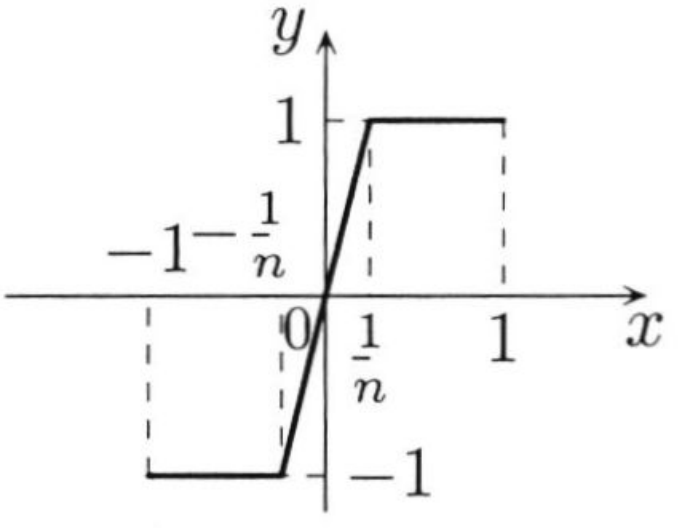
\includegraphics[width=\linewidth]{pic1.png}
	\end{figure}
\end{minipage}
~
\begin{minipage}{0.6\linewidth}
Легко видеть, что
\[
	\forall x \in [0,1] \rightarrow \lim\limits_{n \rightarrow \infty} f_n(x) = \text{sign }x = f(x)  
\]
Докажем, что имеет место сходимость также в среднем квадратичном($ \text{sign }x \in \mathcal{L}_R^2[-1,1 $). В самом деле,
\begin{multline*}
	||f_n - f||_2^2 = \int_{-1}^1 (f_n(x) - f(x))^2dx =\\= 2\int_{0}^{\frac{1}{n}}(1-nx)^2dx < 2\int_{0}^{\frac{1}{n}}1dx = \dfrac{2}{n} \rightarrow 0
\end{multline*}
то есть $ ||f_n-f||_2 \rightarrow0 $
\end{minipage}
\end{greyProof}
\begin{greyEmpty}
Поэтому последовательность $ f_n $ фундаментальна в $ \mathcal{L}_R^2[-1,1] $, значит, и в $ \mathcal{L}_C^2[-1,1] $. Но она не может сходиться в $ \mathcal{L}_C^2[-1,1] $, так как не существует непрерывной на $ [-1,1] $ функции $ g $ такой, что $ ||f_n-g||_2 \rightarrow 0 $.В самом деле, если $ f_n \rightarrow g $ в $ \mathcal{L}_C^2[-1,1] $, то $ f_n \rightarrow g $ в $ \mathcal{L}_R^2[-1,1]$. Так как последовательность $ f_n $ имеет в $ \mathcal{L}_R^2[-1,1] $ два передела $ f $ и $ g $, то $ f =g $ в $ \mathcal{L}_R^2[-1,1] $, т.е. $ f\sim g $ и $ \int_{-1}^1 (f(x) - g(x))^2 dx = 0 $. Отсюда следует, что $ \int_{0}^1 (f(x)-g(x))^2dx = 0 $. Так как $ f(x) = 1 $ на $ [0,1] $, то $ \int_{0}^1(1-g(x))^2dx = 0 $. Так как функция $ g $ непрерывна на $ [-1,1] $, то $ g(x) \equiv 1 $ на $ [0,1] $.Аналогично $ g(x) \equiv -1 $ на $ [-1,0] $. Полученное противоречие показывает, что фундаментальная последовательность $ f_n $ в $ \mathcal{L}_C^2[-1,1] $ не имеет предела в этом пространстве, т.е. пространство $ \mathcal{L}_C^2[-1,1] $ неполно.
\end{greyEmpty}	
	\newpage
	\section{Непрерывность, интегрируемость и дифференцируемость собственных интегралов, зависящих от параметра.}

\textbf{Начальные условия.} $ \prod = \{ (x,y) \in \mathbb{E}^2: a \leqslant x \leqslant b,\; c \leqslant y \leqslant d \} = [a,b]\times[c,d] $

$ w = f(x,y) $, при каждом фиксированном $  y \in [c,d] $, функция $ w = f(x,y) $ интегрируема на $ [a,b] $ 

$ \forall y \in [c,d]\; J = J(y) = \int_{a}^{b} f(x,y)dx$ --- интеграл зависящий от параметра.
\begin{greyTheorem}
	Если $ w = f(x,y) $ непрерывна на $ \Pi $, то функция $ J=J(y) $ непрерывна на $ [c,d] $
\end{greyTheorem}
\begin{greyProof}
	$ \Pi $ --- компакт, $ w = f(x,y) $ непрерывна на $ \Pi $, следовательно можем воспользоваться Т. Кантора: \[
	\forall\varepsilon> 0 \exists 
	\delta=\delta(\varepsilon)>0: \forall (x,y) \in \Pi : y+ \Delta y \in [c,d] \& |\Delta y| < \delta \mapsto |f(x,y+ \Delta y) - f(x,y)| <\dfrac{\varepsilon}{b-a}
	\]
	Рассмотрим приращение функции $ \mathcal{J},\; \forall y \in [c,d] $:
	\begin{multline*}
	\abs{\Delta \mathcal{J}(y, \Delta y)} = \abs{ \mathcal{J}(y+\Delta y)-\mathcal{J}(y)} = \abs{\int_{a}^{b}\left[ f(x,y+\Delta y) - f(x,y) \right]dx} \leqslant \\ \leqslant \int_{a}^{b}\abs{f(x,y+\Delta y) - f(x,y)} dx <\dfrac{\varepsilon}{b-a} \int_{a}^{b} dx = \varepsilon
	\end{multline*}
	$ \Rightarrow \mathcal{J} $ непрерывна на $ [c,d] $
\end{greyProof}
\begin{greyTheorem}
	Если $ w = f(x,y) $ непрерывна на $ \Pi $, то $ \mathcal{J}=\mathcal{J}(y) $ непрерывна на $ [c,d] $ и $ \forall y_o \in [c,d] $ выполняется \[
	\int_{c}^{y_0} \mathcal{J}(y)dy = \int_{c}^{y_0} \left[ \int_{a}^{b} а(x,y)dx \right] dy = \int_{a}^{b} \left[ \int_{c}^{y_0} f(x,y) dy \right] dx
	\]
\end{greyTheorem}
\begin{greyProof}
	Из т. 14.1 следует, что $ \mathcal{J} = \mathcal{J}_y $ интегрируема на $ [c,d] $. По теореме о сведении кратного интеграла к повторному: 
	каждый из повторных интегралов существует и равен двойному интегралу:
	\[
	\iint_{\Pi_0} f(x,y) dxdy\text{, где } \Pi_0 = [a,b] \times [c,d]
	\]
\end{greyProof}
\begin{greyTheorem}
	Если функция $ w = f(x,y) $ и $ w = \Pdd{f}{y}(x,y) $ непрерывна на $ \Pi $, то $ \mathcal{J} = \mathcal{J}(y) $ дифференцируема на $ [c,d] $ и \[
	\mathcal{J}'(y) = \int_{a}^{b} \Pdd{f}{y}(x,y)dx
	\]
\end{greyTheorem}
\begin{greyProof}
	По условию $ w = \Pdd{f}{y}(x,y) $ непрерывна на $ \Pi $ введем функцию $ g(y) = \int_{a}^{b} \Pdd{f}{y}(x,y)dx$ --- непрерывна на $[c,d]$ по т. 14.1 	и интегрируема на $ [c,d] $ по теореме 14.2, следовательно 
	\[
	\forall y \in [c,d] \mapsto \int_{y}^{c} g(y)dy = \int_{a}^{b} \left[ \int_{c}^{y} \Pdd{f}{y}(x,y)dx \right] dy = \int_{a}^{b}\left[ f(x,y) - f(x,c) \right] dx = \mathcal{J}(y) - \mathcal{J}(c)
	\]
	\[
	\mathcal{J}(y) = \int_{c}^{y} g(y)dy + \mathcal{J}(c)
	\]
	Из непрерывности и интегрируемости $ g(y) $, следует дифференцируемость $ \mathcal{J} $ на $ [c,d] $, значит, $  $
	\[
	\mathcal{J}'(y) = g(y) = \int_{a}^{b} \Pdd{f}{y} dx
	\]
\end{greyProof}
%\subsubsection{Интегралы с переменными границами}
%Область $ D $ элементарна относительно Ox: $ \overline{D} = \{ (x,y): a(y)\leqslant x\leqslant b(y),\; y \in [c,d] \} $
%
%Предположим, что $ \forall y \in [c,d] $ функция $ w = f(x,y) $ интегрируема на $ [a(y),b(y)] $, тогда для любого $ y $ определена функция \[
%\mathcal{J} = \mathcal{J}(y) = \int_{a(y)}^{b(y)} f(x,y)dx
%\]
%\begin{theorem}
%	Если функция $ w = f(x,y) $ непрерывна в $ \overline{D} $, а функции $ a = a(y) $ и $ b = b(y) $ непрерывны на $ [c,d] $, то функция $ \mathcal{J} = \mathcal{J}(y) $ непрерывна на $ [c,d] $
%\end{theorem}
%\begin{proof}
%	Фиксируем точку $ y_0 \in [c,d] $, тогда используя свойство аддитивности определенного интеграла можем записать \[
%	\mathcal{J}(y) = \int_{a(y_0}^{b(y_0)}f(x,y)dx + \int_{b(y_0)}^{b(y)}f(x,y)dx - \int_{a(y_0)}^{a(y)} f(x,y)dx = \mathcal{J}_0 + \mathcal{J}_b - \mathcal{J}_a
%	\]
%	$ \mathcal{J}_0 $ непрерывна на $ [c,d] $ по т. 2.1.1. 
%	\[
%	\mathcal{J}_0(y) \underset{y \rightarrow y_0}{=} \mathcal{J}_0 (y_0) = \int_{a(y_0)}^{b(y_0)} = \mathcal{J}(y_0)
%	\]
%	$ \max |f(x,y) | = m,\; \forall x,y \in \overline{D} $
%	\[
%	\abs{\mathcal{J}_0(y)} = \abs{ \int_{a(y)}^{b(y)} f(x,y) dx} \leqslant M \abs{b(y) - b(y_0)} \underset{y \rightarrow y_0}{\longrightarrow} 0 
%	\]
%	для $ \mathcal{J}_a(y) $ аналогично
%\end{proof}
%\begin{theorem}
%	Пусть $ w = f(x,y) $ и $ w = \Pdd{f}{y}(x,y) $ непрерывны в $ \overline{D} $, а функции $ a = a(y) $  и $ b = b(y) $ дифференцируемы на $ [c,d] $, тогда $ \mathcal{J} = \mathcal{J}_y $ дифференцируема на $ [c,d] $ и справедлива формула \[
%	\mathcal{J}'(y) = \int_{a(y)}^{b(y)} \Pdd{f}{y}(x,y)dx + f(b(y),y)b'(y) - f(a(y),y)a'(y)
%	\]
%	По т. 2.1.3 $ \mathcal{J}_0 $ дифференцируема на $ [c,d] $, тогда 
%	\[
%	\mathcal{J}'_0(y) = \int_{a(y_0)}^{b(y_0)} \Pdd{f}{y} (x,y)dx
%	\]
%	\[
%	\mathcal{J}_b(y_0) = \mathcal{J}_a(y_0) = 0 
%	\]
%	\[
%	\mathcal{J}'_b(y_0) = \lim\limits_{y \rightarrow y_0}  \dfrac{\int_{b(y_0)}^{b(y)} f(x,y)dx}{y - y_0} 
%	\]
%	по интегральной теореме о среднем $ \exists \overline{x} \in (b(y_0),b(y) $:
%	\[
%	\lim\limits_{y\rightarrow y_0}	f(\overline{x},y) \dfrac{b(y) - b(y_0)}{y - y_0}
%	\] 
%	при $ y \rightarrow y_0 \; \overline{x} \rightarrow y_0$, тогда выражение выше равно 
%	\[
%	f(b(y_0),y_0) b'(y_0)
%	\]
%	Аналогично для $ \mathcal{J}_a(y_0) $
%\end{theorem}
	
	\newpage
	\section{Равномерная сходимость несобственных интегралов, зависящих от параметра. Критерий Коши, признаки Вейерштрасса и Дирихле.}

\textbf{Несобственный интеграл первого рода. Начальные условия.}

%\textbf{В нашем курсе мы не сталкиваемся с интегралами первого рода, так что это просто для справки.}
$ \Pi - [a, + \infty)\times E $, где $ E \in \mathbb{R}^1 $

$ w = f(x,y)$ при каждом фиксированном $ y \in E $ интегрируема в несобственном смысле на $ [a,+\infty) $\[
\mathcal{J} = \mathcal{J}_y = \int_{a}^{+ \infty} f(x,y)dx,\; y \in E
\]
\begin{greyDefinition} Несобственный интеграл $ \mathcal{J} = \mathcal{J}_y $ сходится равномерно по параметру $ y $ на множестве $ E $, если
\[
\forall \varepsilon > 0 \exists A = A (\varepsilon) \geqslant a: \forall R \geqslant A \& \forall y \in E \mapsto \abs{ \int_{R}^{+ \infty} f(x,y) dx} < \varepsilon
\]
\textbf{Отрицание:}
\[
\exists \varepsilon_0 > 0 : \forall A \geqslant a \exists R_A \geqslant A \& \exists y_a \in E \mapsto \abs{\int_{R_A}^{+\infty}f(x,y_A)}\geqslant \varepsilon_0
\]
\end{greyDefinition}
\textbf{Несобственный интеграл второго рода. Начальные условия.}
$ \Pi_b = [a,b)\times E, \in \subset \mathbb{R} $

Если $ \forall y \in E $ фиксированная функция $ w = f(x,y) $ интегрируема в несобственном смысле на $ [a,b) $, то на $ E $ определена функция: \[
\mathcal{J} = \mathcal{J}(y) = \int_{a}^{b} f(x,y)dx
\]
\begin{greyDefinition} Несобственный интеграл $ \mathcal{J} = \mathcal{J}(y) $ сходится равномерно по параметру $ y $ на $ E $
\[
\forall \varepsilon > 0 \; \exists  \delta=\delta(\varepsilon) > 0 : \forall \eta \in (0,\delta) \;\&\; \forall y \in E \mapsto \abs{\int_{b-\eta}^{b} F(x,y)dx } < \varepsilon
\]
\end{greyDefinition}
\begin{greyTheorem}\textbf{Критерий Коши.}
	Для равномерной сходимости по параметру $ y $ на множестве $ E $ несобственного интеграла $ \mathcal{J} = \mathcal{J}(y) $ необходимо и достаточно, чтобы выполнялось следующее условие:\begin{multline*}
	\forall \varepsilon > 0 \exists A = A(\varepsilon) > 0 >\geqslant a: \forall R', R'': R'' > R' \geqslant A \& \forall y \in E \mapsto \\ \mapsto | \int_{ R' }^{ R'' } f(x,y) | < \varepsilon
	\end{multline*}
\end{greyTheorem}
\begin{greyProof}
	\textit{Необходимость.}
	
	Непосредственно следует из определения.
	\begin{multline*}
		\forall \varepsilon > 0 \exists A = A((\varepsilon) \geqslant a: \forall R' \geqslant A \und \forall y \in E \mapsto \\ \mapsto \left| \int_{ R' }^\infty f(x,y)dx \right| < \dfrac{\varepsilon}{2},\; \left| \int_{ R''}^\infty f(x,y)dx \right| < \dfrac{\varepsilon}{2}
	\end{multline*}
	Так как $ R'' > R' \Rightarrow \left| \int_{ R' }^{R''} f(x,y)dx \right| < \varepsilon$
	
	\textit{Достаточность.}
	\[
	\forall \varepsilon > 0 \exists A = A(\varepsilon) > 0 >\geqslant a: \forall R', R'': R'' > R' \geqslant A \& \forall y \in E \mapsto | \int_{ R' }^{ R'' } f(x,y) | < \varepsilon
	\]
	Тогда по критерию Коши сходимости несобственных интегралов при всех $ y \in E $ интеграл сходится, следовательно устремляя $ R^n \rightarrow \infty $ получаем равномерную сходимость.
\end{greyProof}
\begin{greySmth}{Замечание}
\textbf{Отрицание условия Коши:}\[
\exists \varepsilon_0 > 0 : \forall A \geqslant a \;\exists R'_A, R''_A: R''_A > R'_A \geqslant A \;\&\; \exists y_A \in E: \abs{ \int_{R'_A}^{R_A''} f(x,y_A)dx} \geqslant \varepsilon_0
\]
\end{greySmth}
\begin{greyTheorem}\textbf{Признак Вейерштрасса.}
	Функция $ w = f(x,y) $ определена на $ \Pi = [a, +\infty)\times E $, при каждом фиксированном $ y \in E $ функция $ f $ интегрируема на $ [a,R],\;\forall R > a$ и на $ \Pi $ выполнено неравенство $ \abs{f(x,y)} \leqslant g(x) $. Если $ \int_{a}^{+\infty} g(x) dx < \infty$, то несобственный интеграл $ \mathcal{J} = \mathcal{J}(y)  $ сходится равномерно по параметру $ y $ на $ E $
\end{greyTheorem}
\begin{greyProof}
	Из критерия Коши:
	\[
	\int_{a}^{+ \infty} g(x)dx < \infty \Leftrightarrow \forall \varepsilon > 0\; \exists A= A(\varepsilon): \forall R', R'': R' > R'' \geqslant A \mapsto \int_{ R' }^{R''} g(x)dx < \varepsilon
	\] 
	Тогда $ \forall y \in E $ выполняется 
	\[
	\abs{\int_{ R' }^{R''}f(x,y) dx} \leqslant \int_{ R' }^{R''}\abs{f(x,y)}dx \leqslant \int_{ R' }^{R''} g(x)dx < \varepsilon
	\]
	Следовательно $ \mathcal{J}=\mathcal{J}(y) $ сходится равномерно по параметру $ y $ на $ E $
\end{greyProof}	
\begin{greySmth}{Следствие.} Если функция $ w = \varphi(x,y) $ ограничена на $ \Pi = [a,+\infty)\times E $ и \newline $ \forall y \in E \; \varphi(x,y)$ интегрируема на $ [a,R]\; \forall R\geqslant a $ , а $ \int_{a}^{+\infty} |h(x)|dx < \infty $, то сходится равномерно по параметру $ y $ на $ E $ интеграл $	\int_{a}^{b} \varphi(x,y)h(x)dx
$
\end{greySmth}
\begin{greyProof}
	\[
	g(x) = M |h(x)|,\; M = \sup_\Pi \abs{\varphi(x,y)} \Rightarrow \text{ признак Вейрештрасса.}
	\]
\end{greyProof}
\begin{greyTheorem}\textbf{Признак Дирихле.} Пусть $ w = f(x,y) $ непрерывна в $ \Pi_\infty $ и $ \forall x \in [c.d] \; \mathcal{J}(y) = \int_{a}^{+\infty}f(x,y)dx $ сходится и выполнены следующие условия:
	\begin{enumerate}
		\item  $ \exists M > 0 : \forall R > a \und \forall y \in [c,d]\; \left|\int_{R}^{\infty} f(x,y)dx \right| \leqslant M $
		\item $ g = g(x) $ непрерывно дифференцируема, монотонна и $$ g(x) \underset{x \rightarrow +0}{\longrightarrow} 0,$$ 
		Тогда $ \int_{a}^{b} f(x,y)g(x)dx$  сходится равномерно по параметру $ y $ на $ [c,d] $
	\end{enumerate}
\end{greyTheorem}
\begin{greyProof}
	Проинтегрируем по частям: $\forall R > a \und \forall y \in [c,d] \mapsto$
	\[
		\mapsto \int_{ R}^{+\infty} f(x,y)g(x)dx = F(x,y)g(x) \Big|_{R}^{+\infty} - \int_{ R}^{+\infty} F(x,y)g'(x)dx
	\]
\end{greyProof}
\begin{greyEmpty}
	Так как $ \forall y \in [c,d] \mapsto \lim\limits_{x \rightarrow + \infty } F(x,y)g(x) = 0 \Rightarrow $
	\[
	\Rightarrow \int_R^{+\infty} f(x,y)g(x0dx = - F(R,y)g(R) - \int_{ R}^{+\infty}F(x,y)g'(x)dx;
	\]
	По условию $ g'(x) \leqslant 0 \und \lim\limits_{x \rightarrow + \infty } g(x) = 0 \Rightarrow g(R) \geqslant 0$ и опять же по условию $ \abs{\int_{ R}^{+\infty}f(x,y)dx} \leqslant M \Rightarrow $
	\[
		\abs{\int_{ R}^{+\infty} f(x,y)g(x)dx} \leqslant Mg(R) - M \int_{ R}^{+\infty} g'(x)dx = 2Mg(R) = 2M \abs{g(R)}
	\] 
\end{greyEmpty}
\begin{greyTheorem}\textbf{Признак Дини.}
	Пусть функция $ w = f(x,y) $ непрерывна на $ \Pi_\infty $, неотрицательна на нем и $ \forall y \in [c,d] $ интеграл $ \mathcal{J}(y)  $ сходится и функция $ \mathcal{J}(y) $ непрерывна на $ [c,d] $, тогда $ \mathcal{J}(y) $ сходится равномерно по параметру $ y $ на $ [c,d] $.
\end{greyTheorem}	
\end{document}